\documentclass[oneside]{VUMIFPSkursinis}
\usepackage{algorithmicx}
\usepackage{algorithm}
\usepackage{algpseudocode}
\usepackage{amsfonts}
\usepackage{float}
\usepackage{amsmath}
\usepackage{bm}
\usepackage{caption}
\usepackage{color}
\usepackage{float}
\usepackage{graphicx}
\usepackage{listings}
\usepackage{subfig}
\usepackage{ltablex}
\usepackage{longtable}
\usepackage{wrapfig}
\usepackage{subfig}
\usepackage{pbox}
\renewcommand{\labelenumii}{\theenumii}
\renewcommand{\theenumii}{\theenumi.\arabic{enumii}.}
\renewcommand{\labelenumiii}{\theenumiii}
\renewcommand{\theenumiii}{\theenumii\arabic{enumiii}.}
\newcolumntype{P}[1]{>{\centering\arraybackslash}p{#1}}
\usepackage[%  
    colorlinks=true,
    linkcolor=black
]{hyperref}
\university{Vilniaus universitetas}
\faculty{Matematikos ir informatikos fakultetas}
\department{Programų sistemų katedra}
\papertype{Programų sistemų inžinerija II laboratorinis darbas I}
\title{Reikalavimų apibrėžimas}
\titleineng{Requirements specification}
\status{2 kurso 3 grupės studentai}



\supervisor{Audronė Lupeikienė, M. Darbuot., Dr.}
\date{Vilnius – \the\year}

\bibliography{bibliografija}

\begin{document}
\maketitle
\tableofcontents

\section{Autoriai}
	\begin{itemize}
		\item Matas Savickis
		\item Greta Pyrantaitė
		\item Justas Tvarijonas
		\item Rytautas Kvašinskas
		\item Tomas Kiziela
	\end{itemize}
\section{Įžanga}
Mūsų komanda gavo kitos komandos pirmame semestre(PSI I) paruoštą slidinėjimo kurorto projektą. Šiame darbe sieksime toliau plėtoti ir keisti šį projektą. Toliau vystant projektą keisis dauguma dalių. Siekiant padaryti gerą produktą kai kurios  dalys bus pašalintos ir pridėtos naujos. Pirmame semestre projektuojant dėmesys buvo skiriamas klasikinei projektavimo paradigmai. Šiame darbe projektą rašysime pasinaudodami ICONIX principu, projektuojant dėmesys bus skiriamas GUI sudarymui ir iš to išplauks sistemos projektavimas ir sandara. 

\section{Reikalavimai}
Šioje dalyje bus pateikti funkciniai bei nefunkciniai reikalavimai sistemai. Stengsimės prisilaikyti ,,užsakovų"(grupės, iš kurios gavome jų darbą) reikalavimus, tačiau siekiant sukurti geresnę sistemą pridėsime kai kuriuos savo sugalvotus reikalavimus arba ignoruosime mums pateiktus reikalavimus. 

\subsection{Reikalavimų pataisymai}
	\begin{itemize}
		\item{X - ištrintas}
		\item{M - pakeistas}
		\item{N - nekeistas}
	\end{itemize}

%\begin{table}[HTTP]

\begin{longtable}{ | p{0.04\textwidth}|p{0.43\textwidth}|p{0.09\textwidth}|p{0.15\textwidth}|p{0.21\textwidth}| }  \hline
	Nr. & Pradinis reikalavimas&  Pakeitimo tipas & Klaidos aprašas  & Naujas reikalavimas \\ \hline
	FR & ,,Žetonas" seka vartotojo laiką praleistą trasoje & M & Pakeistas neaiškus daiktavardis & Sekimo prietaisas seka vartotojo laiką praleistą trasoje \\ \hline	
	FR & Vartotojo prieigos prie pramogų prieinamumas nustatomas naudojant pirštų antspaudą & M & Sukonkretintas abstraktus reikalavimas & Vartotojui norint pasinaudoti kavinės paslaugomis naudojamas piršto antspaudas \\ \hline
	FR &  Sistema leidžia vartotojui už paslaugas atsiskaityti e-bankininkyste & N & - & - \\ \hline
	FR & ,,Žetonas" skaičiuoja greičiausią laiką, per kurį vartotojas įveikia trasą & M & Pakeistas neaiškus daiktavardis & Sekimo prietaisas fiksuoja greičiausią laiką, per kurį vartotojas įveikė trasą \\ \hline
	FR & Vartotojo trasų laikai rodomi internetinėje aplikacijoje & N & - & - \\ \hline
	FR & Sistema seka vartotojų poziciją specialaus žetono pagalba, kurį gauna kiekvienas vartotojas apsilankęs kurorte(vieta sekama tik gavus vartotojo sutikimą) & M & Reikalavimas skliausteliuose turėtų būti perkeltas į nefunkcinius (pvz. saugumo) raiklavimus & Sistema seka vartotojo poziciją specialaus sekimo prietaiso pagalba, kurį gauna kiekvienas apsilankęs kurorte \\ \hline
	FR & 3.1.1. Sukurti raktą naujos esybės registracijai
FR 1. Pradiniai duomenys:
FR 1.1. Nėra.
FR 2. Veiksmai:
FR 2.1. Atidaryti formą;
FR 2.2. Įvesti slaptažodį;
FR 2.3. Spausti mygtuką „Generuoti raktą“.
FR 3. Alternatyvūs scenarijai:
FR 3.1. Esybė įveda neteisingą slaptažodį, tada išvedamas pranešimas apie nesėkmingą užklausą.
FR 4. Reikalavimai:
FR 4.1. Esybė gali generuoti raktą tik vienodą vaidmenį turinčiai esybei.
FR 5. Rezultatas:
FR 5.1. Sugeneruotas slaptažodis (raktas) išvedamas tekstiniame lauke. & X & Reikalavimai išmetami, nes neprideda jokios naudos dokumentacijos skaitytojui ir yra nefunkciniai. & - \\ \hline
    FR & 3.1.2. Sukurti naujos esybės paskyrą
FR 6. Pradiniai duomenys:
FR 6.1. Vardas (1-64 simboliai);
FR 6.2. Pavardė (1-64 simboliai);
FR 6.3. El. paštas (iki 64 simbolių);
FR 6.4. Slaptažodis (nuo 10 simbolių iki 64 simbolių, turi būti panaudota bent po vieną didžiąją, mažąją raidę, skaitmenį ir specialų simbolį (*,\#,- ir tt).
FR 6.5. Raktas.
FR 7. Veiksmai:
FR 7.1. Meniu juostoje spaudžiama nuoroda „Registration”;
FR 7.2. Išskleistame meniu pasirenkamas esybės tipas;
FR 7.3. Atsidariusioje formoje įrašomas raktas;
FR 7.4. Atsidariusioje registracijos formoje visi laukeliai užpildomi duomenimis;
FR 7.5. Spaudžiamas mygtukas „Sign up“.
FR 8. Alternatyvūs scenarijai:
FR 8.1. Įvedus neteisingą raktą, išvedamas pranešimas apie tai;
FR 8.2. Įvedus negaliojantį raktą, išvedamas pranešimas apie tai.
FR 9. Reikalavimai:
FR 9.1. Raktas turi būti nesenesnis negu 15 minučių;
FR 9.2. Sistema turi patikrinti rakto validumą;
FR 9.3. Visi registracijos laukai turi būti užpildyti;
FR 9.4. Įvedamas slaptažodis negali būti matomas;
FR 9.5. Negalima užsiregistruoti su jau naudojamu el. paštu.
FR 10. Rezultatai:
FR 10.1. Sukuriama esybės paskyra;
FR 10.2. Atidaroma prisijungimo forma. & X & Šie reikalavimai yra nefinkciniai, todėl pašalinami. & - \\ \hline
     FR & 3.1.3. Rezervuoti slidinėjimo objektą
FR 11. Pradiniai duomenys
FR 11.1. Nuomojami objektai
FR 11.2. Telefono numeris
FR 11.3. Slidinėtojų skaičius
FR 11.4. Rezervacijos laikotarpis
FR 11.5. Asmeniniai pageidavimai
FR 12. Veiksmai
FR 12.1. Vartotojas meniu juostoje paspaudžia ant mygtuko “Reservation”;
FR 12.2. Vartotojas pasirenka pradinę bei galutinę rezervacijos datą;
FR 12.3. Vartotojas pasirenka objektų kategorijas iš pateikiamo sąrašo;
FR 12.4. Vartotojas pasirenka konkrečius objektus iš pateiktų objektų lentelių
FR 13. Alternatyvūs scenarijai
FR 13.1. Jei vartotojas neprisijungęs, išmetamas prisijungimo puslapis;
FR 13.2. Jei slidinėjimo objektų sąrašas tuščias, apie tai išmetamas pranešimas;
FR 13.3. Jei administratorius nepatvirtina rezervacijos, apie tai informuojamas vartotojas;
FR 14. Reikalavimai
FR 14.1. Vartotojas turi būti prisijungęs;
FR 14.2. Galutinė data turi būti ne mažesnė nei pradinė data;
FR 14.3. Turi būti netuščias slidinėjimo objektų sąrašas;
FR 15. Rezultatai
FR 15.1. Vartotojas išsiunčia užklausą;
FR 15.2. Vartotojas gauna patvirtinimą, kad rezervacija sėkmingai patvirtinta. & M & Per daug detalūs, reikia apibendrint ir performuluoti. & Vartotojas turi galimybę užrezervuoti slidinėjimo takelį nurodant: nuomojamus objektus, telefono numerį, slidinėtojų skaičių, rezervacijos laikotarpį ir asmeninius pageidavimus. \\ \hline
    FR & 3.1.4. Pasižiūrėti informaciją apie slidinėjimo objektą
FR 16. Pradiniai duomenys
FR 16.1. Slidinėjimo objektas
FR 17. Veiksmai
FR 17.1. Vartotojas meniu juostoje paspaudžia ant mygtuko “Objects Information“;
FR 17.2. Parodomas sąrašas;
FR 17.3. Vartotojas pasirenka objektą iš pateikiamo sąrašo;
FR 18. Alternatyvūs scenarijai
FR 18.1. Jei vartotojas neprisijungęs, išmetamas prisijungimo puslapis;
FR 18.2. Jei slidinėjimo objektų sąrašas tuščias, parodomas pranešimas;
FR 19. Reikalavimai
FR 19.1. Vartotojas turi būti prisijungęs;
FR 19.2. Turi būti netuščias slidinėjimo objektų sąrašas;
FR 20. Rezultatai
FR 20.1. Vartotojas gauna informaciją apie slidinėjimo objektą (rūšis, prieinamą kiekį, nuomos kainą). & M & Reikia sutrumpinti ir performuluoti reikalavimus. & Vartotojas gali matyti informaciją apie slidinėjimo objektą: rūšis, prieinamas kiekis, nuomos kaina, užimtumas nurodytu laiko tarpu.\\ \hline
    FR & 3.1.5. Pasižiūrėti slidinėjimo objekto užimtumą
FR 21. Pradiniai duomenys
FR 21.1. Laikotarpis;
FR 21.2. Slidinėjimo objektas.
FR 22. Veiksmai
FR 22.1. Vartotojas meniu juostoje paspaudžia ant mygtuko “Objects usage“;
FR 22.2. Pasirenka laikotarpį;
FR 22.3. Vartotojas pasirenka objektą iš pateikiamo sąrašo ;
FR 23. Alternatyvūs scenarijai
FR 23.1. Jei vartotojas neprisijungęs, išmetamas prisijungimo puslapis;
FR 24. Reikalavimai
FR 24.1. Turi būti netuščias slidinėjimo objektų sąrašas;
FR 24.2. Vartotojas turi būti prisijungęs;
FR 25. Rezultatai
FR 25.1. Vartotojas gauna informaciją apie slidinėjimo objektą (rūšis, likutį, nuomos kainą). & X &  Galima sujungti šį reikalavimą su prieš tai buvusiu, kur nurodoma informacija apie slidinėjimo objektą. & - \\ \hline
	FR & 3.1.6. Atsijungimas
FR 26. Pradiniai duomenys
FR 26.1. Nėra
FR 27. Veiksmai
FR 27.1. Vartotojas meniu juostoje paspaudžia ant mygtuko “Log out”;
FR 28. Alternatyvūs scenarijai
FR 28.1. Jei vartotojas yra rezervacijos lange, jo paklausiama, ar tikrai nori atsijungti/
FR 29. Reikalavimai
FR 29.1. Vartotojas turi būti prisijungęs;
FR 30. Rezultatai
FR 30.1. Vartotojas atsijungia ir jam parodomas pirminis langas & M & Apibendrinamas reikalavimas & Vartotojas turi galėti atsijungti nuo sistemos\\ \hline
FR & 3.1.7. Atnaujinti slaptažodį
FR 31. Pradiniai duomenys
FR 31.1. E-paštas.
FR 32. Veiksmai
FR 32.1. Vartotojas meniu juostoje paspaudžia ant mygtuko “Forgot Password”;
FR 32.2. Vartotojas suveda savo E-paštą ir paspaudžia ant mygtuko “New Password”;
FR 32.3. Vartotojui išsiunčiamas naujas sugeneruotas slaptažodis.
FR 33. Reikalavimai
FR 33.1. Vartotojas turi būti atsijungęs;
FR 34. Rezultatai
FR 34.1. Vartotojas parodomas prisijungimo puslapis & M & Apibendrinamas reikalavimas & Vartotojas turi galėti atnaujinti slaptažodį\\ \hline
	FR & 3.2.1. Pasižiūrėti orus
FR 35. Pradiniai duomenys
FR 35.1. Data;
FR 36. Veiksmai
FR 36.1. Vartotojas meniu juostoje paspaudžia ant mygtuko „Weather“;
FR 36.2. Vartotojas pasirenka dieną, kurios orų prognozę nori sužinoti;
FR 37. Alternatyvūs scenarijai
FR 37.1. Jei data mažesnė, nei dabartinė diena, parodoma klaida;
FR 37.2. Jei orų prognozės nėra duomenų bazėje, parodomas pranešimas;
FR 38. Reikalavimai
FR 38.1. Data turi būti ne mažesnė nei dabartinė diena;
FR 38.2. Orų prognozė pasirinktai dienai turi būti duomenų bazėje;
FR 39. Rezultatai
FR 39.1. Vartotojui pateikiama orų prognozė; & M & Apibendrinamas reikalavimas & Vartotojas turi galėti pasižiūrėti orus\\ \hline
	FR & 3.2.2. Parašyti laišką
FR 40. Pradiniai duomenys
FR 40.1. Laiško tema;
FR 40.2. Laiško turinys;
FR 41. Veiksmai
FR 41.1. Vartotojas meniu juostoje paspaudžia ant mygtuko “Mail”;
FR 41.2. Vartotojas parašo laiško temą bei turinį;
FR 41.3. Vartotojas paspaudžia mygtuką “Send”
FR 42. Alternatyvūs scenarijai
FR 42.1. Jei vartotojas neprisijungęs, išmetamas prisijungimo puslapis;
FR 42.2. Jei tema ar turinys tuščias, laukelis paraudonuoja ir laiškas nėra išsiunčiamas;
FR 43. Reikalavimai
FR 43.1. Vartotojas turi būti prisijungęs;
FR 43.2. Turinys bei tema neturi būti tušti;
FR 43.3. Temos ilgis neturi viršyti 50 simbolių;
FR 43.4. Turinio ilgis neturi viršyti 500 simbolių;
FR 44. Rezultatai
FR 44.1. Vartotojui pranešama, jog laiškas sėkmingai išsiųstas; & M & Apibendrinamas reikalavimas & Vartotojas turi galėti parašyti laišką \\ \hline

	FR & 3.3.1. Parašyti ataskaitą
FR 45. Pradiniai duomenys
FR 45.1. Ataskaitos pavadinimas;
FR 45.2. Ataskaitos turinys;
FR 46. Veiksmai
FR 46.1. Darbuotojas meniu juostoje paspaudžia ant mygtuko “Reports”;
FR 46.2. Darbuotojas parašo ataskaitos pavadinimą bei turinį;
FR 46.3. Darbuotojas paspaudžia mygtuką “Send”
FR 48. Reikalavimai
FR 48.1. Darbuotojas turi būti prisijungęs;
FR 48.2. Pavadinimas bei tema neturi būti tušti;
FR 48.3. Pavadinimo ilgis neturi viršyti 50 simbolių;
FR 48.4. Turinio ilgis neturi viršyti 500 simbolių;
FR 49. Rezultatai
FR 49.1. Darbuotojui pranešama, jog ataskaita sėkmingai išsiųstas. & M & Apibendrinamas reikalavimas & Vartotojas turi galėti parašyti ataskaitą\\ \hline
FR & 
FR 93. Pradiniai duomenys: 
FR 93.1. Objekto kategorija(-os). 
FR 94. Veiksmai: 
FR 94.1. Meniu juostoje paspaudžiama ant mygtuko „Set the object state”;
 FR 94.2. Iš objektų kategorijų sąrašo (kambarys, slidinėjimo trasa, slidinėjimo įranga) pasirenkama viena kategorija;
 FR 94.3. Parodomas sąrašas objektų, priklausančių tai kategorijai;
 FR 94.4. Pasirenkamas vienas objektas; FR 94.5. Pasirenkama data;
 FR 94.6. Pažymima būsena, paspaudžiant ant mygtuko „Set the state”.
 FR 95. Alternatyvūs scenarijai:
 FR 95.1. Nutrūko ryšys su duomenų baze.
 FR 96. Reikalavimai: 
FR 96.1. Administratorius turi būti prisijungęs.
 FR 97. Rezultatai:
 FR 97.1. Duomenų bazėje pažymima objekto būsena. 
& M & Apibendrinamas reikalavimas & Sistema administratoriui suteikia galimybę stebėti duombazės objektų būseną. \\ \hline
FR & 3.4.4. Peržiūrėti statistiką
FR 58. Pradiniai duomenys
FR 58.1. Laikotarpis, kurio duomenis savininkas nori gauti;
FR 58.2. Duomenų tipas (klientų srautas ir/arba pajamos)
FR 59. Veiksmai
FR 59.1. Pasirinkti duomenų tipą;
FR 59.2. Pasirinkti laikotarpį;
25
FR 59.3. Spausti mygtuką „Get data”
FR 60. Alternatyvūs scenarijai:
FR 60.1. Pasirinktam laikotarpiui nėra įrašų duomenų bazėje, tada išvedamas pranešimas apie tai.
FR 61. Reikalavimai:
FR 61.1. Savininkas privalo būti prisijungęs prie savo paskyros;
FR 61.2. Būtina pasirinkti egzistuojantį laikotarpį (tai reiškia negali data “nuo” būti vėliau negu data “iki”);
FR 62. Rezultatas:
FR 62.1. Diagramoje pavaizduojami pasirinkti duomenys. & M &  Apibendrinamas reikalavimas & vartotojas turi galėti peržiūrėti statistiką. \\ \hline
FR & 3.4.5. Peržiūrėti paslaugų ar įrangos tiekėjų sąrašą
FR 63. Pradiniai duomenys
FR 63.1. Paslaugų tipas(-ai) (įranga, elektros energija, šilumos energija, apsaugos tarnyba);
FR 63.2. Laikotarpis, kurio duomenis savininkas nori gauti;
FR 64. Veiksmai:
FR 64.1. Pasirinkti paslaugų tipą(-us);
FR 64.2. Pasirinkti laikotarpį (gali būti tuščias);
FR 64.3. Spausti mygtuką „See suppliers”;
FR 65. Alternatyvūs scenarijai:
FR 65.1. Pasirinktai paslaugai nėra apibrėžtas tiekėjas, tada išvedamas pranešimas apie tai;
FR 66. Reikalavimai:
FR 66.1. Savininkas privalo būti prisijungęs prie savo paskyros;
FR 66.2. Būtina pasirinkti bent vieną paslaugą;
FR 66.3. Paslaugos privalo būti pavaizduotos drop-down sąraše;
FR 66.4. Kol nepasirinkta nė viena paslauga, mygtukas yra išjungtas;
FR 67. Rezultatas:
FR 67.1. Pavaizduojamas sąrašas pasirinktų paslaugų tiekėjų. & M &  Apibendrinamas reikalavimas & vartotojas turi galėti peržiūrėti paslaugų ir įrangos tiekėjų sąrašus \\ \hline


FR &  FR 68. Pradiniai duomenys:
FR 68.1. Sutarties pavadinimas;
FR 69. Veiksmai:
FR 69.1. Pasirinkti norimą sutartį;
FR 69.2. Spausti mygtuką „Read the agreement”;
FR 69.3. Alternatyvūs scenarijai:
FR 69.4. Pasirinkta sutartis prieš akimirką buvo nutraukta, ir kitas savininkas pažymi apie tai, tada išvedamas pranešimas apie tai;
FR 70. Reikalavimai:
FR 70.1. Savininkas privalo būti prisijungęs prie savo paskyros;
FR 70.2. Sutartys privalo būti pavaizduotos drop-down sąraše;
FR 70.3. Kol nepasirinkta sutartis, mygtukas yra išjungtas;
FR 70.4. Galima pasirinkti tik vieną sutartį. & M & Reikalavimai padalinti iš nulio & Vartotojas turi galėti peržiūrėti sutartis. \\ \hline

FR & FR 71. Pradiniai duomenys:
FR 71.1. Vartotojo tipas (klientas, darbuotojas, administratorius, savininkas);
FR 71.2. Administratoriaus el. paštas;
FR 71.3. Slaptažodis.
FR 72. Veiksmai:
FR 72.1. Pasirenkamas prisijungimo tipas;
FR 72.2. Įvedami prisijungimo duomenys;
FR 72.3. Spaudžiamas mygtukas „Log in”.
FR 73. Alternatyvūs scenarijai:
FR 73.1. Įvedus neteisingus duomenis, ar palikus bent vieną tuščią laukelį, langeliai pažymimi raudonai ir išvedamas pranešimas dėl neteisingo duomenų įvedimo.
FR 74. Reikalavimai:
FR 74.1. Administratoriaus el. paštas ir slaptažodis turi sutapti su duomenimis, esančiais duomenų bazėje;
FR 74.2. Įvedamas slaptažodis negali būti matomas.
FR 75. Rezultatas:
FR 75.1. Administratorius prisijungia prie savo paskyros;
FR 75.2. Atidaromas pagrindinis puslapis. & M & Kam kilo idėja taip padaryt tokį reikalavimą? & Administratorius turi galėti prisijungti prie savo paskyros. \\ \hline

FR & FR 76. Veiksmai:
FR 76.1. Meniu juostoje paspaudžiama ant mygtuko „Employees”;
FR 77. Alternatyvūs scenarijai:
FR 77.1. Įmonėje niekas nedirba, tada išvedamas pranešimas apie tai.
FR 78. Reikalavimai:
FR 78.1. Darbuotojų sąrašas surikiuotas pareigų svarbos mažėjimo tvarka.
FR 79. Rezultatas:
FR 79.1. Išvedamas darbuotojų sąrašas. & M & Performuluoti ir sutraukti funkciniai reikalavimai & Vartotojas gali peržiūrėti darbuotojų sąrašą. \\ \hline

FR & FR 80. Pradiniai duomenys:
FR 80.1. Darbuotojo ID.
FR 81. Veiksmai:
FR 81.1. Meniu juostoje paspaudžiama ant mygtuko „Modify the list of employees”;
FR 81.2. Paspaudžiamas mygtukas „Add new” ;
FR 81.3. Tekstiniame lauke įrašomas darbuotojo ID;
FR 81.4. Paspaudžiamas mygtukas pridėti.
FR 82. Alternatyvūs scenarijai:
FR 82.1. Darbuotojo ID nėra duomenų bazėje, tada išvedamas pranešimas apie tai ir tekstinis laukas pažymimas raudonai.
FR 83. Reikalavimai:
FR 83.1. Darbuotojo ID turi būti duomenų bazėje;
FR 83.2. Darbuotojų sąrašas turi būti surikiuotas pareigų svarbos mažėjimo tvarka;
FR 83.3. Pridėjus darbuotoją sąrašas iš karto atsinaujina. & M & Performuluoti ir sutraukti funkciniai reikalavimai & Vartotojas turi galimybę pridėti darbuotoją į sistemą. \\ \hline

FR & FR 84. Pradiniai duomenys:
FR 84.1. Darbo sutarties nutraukimo sutartis.
FR 85. Veiksmai:
FR 85.1. Meniu juostoje paspaudžiama ant mygtuko „Modify the list of employees”;
FR 85.2. Paspaudžiamas mygtukas „-”;
FR 85.3. Sąraše pažymimas darbuotojas (galima tik vieną);
FR 85.4. Virš sąrašo pasirodo mygtukas „Remove”;
FR 85.5. Paspaudžiamas virš sąrašo esantis mygtukas „Remove”;
FR 85.6. Po mygtuku „Remove” pasirodo dialogo langas su klausimu „Are you sure?”;
FR 85.7. Spaudžiame mygtuką „Yes”.
FR 85.8. Alternatyvūs scenarijai:
FR 85.9. Dialogo lange paspaudus „No” forma atsinaujina, nė vienas darbuotojas nėra pasirinktas pašalinimui.
FR 86. Reikalavimai:
FR 86.1. Darbuotojų sąrašas turi būti surikiuotas pareigų svarbos mažėjimo tvarka;
FR 86.2. Turi būti papildomas tekstinis laukas, kuris palengvina darbuotojo paiešką (t.y. paieškos laukas);
FR 86.3. Pašalinus darbuotoją iš karto sąrašas atsinaujina.
FR 87. Rezultatas:
FR 87.1. Pasirinktas darbuotojas pašalinamas iš darbuotojų sąrašo. & M & Performuluoti ir sutraukti funkciniai reikalavimai & Vartotojas gali atleisti darbuotojus \\ \hline

FR & FR 88. Pradiniai duomenys:
FR 88.1. Objekto kategorija(-os).
FR 89. Veiksmai:
FR 89.1. Meniu juostoje paspaudžiama ant mygtuko „Check the object state”;
FR 89.2. Iš objektų kategorijų sąrašo (kambarys, slidinėjimo trasa, slidinėjimo įranga) pasirinkti ne mažiau nei vieną kategoriją;
FR 89.3. Pasirinkti datą;
FR 89.4. Paspausti mygtuką „Show states”.
FR 90. Alternatyvūs scenarijai:
FR 90.1. Bent vienoje kategorijoje nėra nė vieno objekto, tada išvedamas pranešimas apie trūkstamus objektus.
FR 91. Reikalavimai:
FR 91.1. Administratorius privalo būti prisijungęs prie paskyros.
FR 92. Rezultatas:
FR 92.1. Lentelėje(-ėse) pavaizduojamos pasirinktų objektų būsenos. & M & I swear to God, whoever came up with these..... & Vartotojas gali peržiūrėti nuomojamų objektų būseną. \\ \hline

FR & FR 93. Pradiniai duomenys:
FR 93.1. Objekto kategorija(-os).
FR 94. Veiksmai:
FR 94.1. Meniu juostoje paspaudžiama ant mygtuko „Set the object state”;
FR 94.2. Iš objektų kategorijų sąrašo (kambarys, slidinėjimo trasa, slidinėjimo įranga) pasirenkama viena kategorija;
FR 94.3. Parodomas sąrašas objektų, priklausančių tai kategorijai;
FR 94.4. Pasirenkamas vienas objektas;
FR 94.5. Pasirenkama data;
FR 94.6. Pažymima būsena, paspaudžiant ant mygtuko „Set the state”.
FR 95. Alternatyvūs scenarijai:
FR 95.1. Nutrūko ryšys su duomenų baze.
FR 96. Reikalavimai:
FR 96.1. Administratorius turi būti prisijungęs.
FR 97. Rezultatai:
FR 97.1. Duomenų bazėje pažymima objekto būseną. & M & Honestly, I'm out of ideas what to put here & Vartotojas gali pakeisti objektų būsenas duomenų bazėje. \\ \hline


FR & 
FR 98. Pradiniai duomenys: 
FR 98.1. Ataskaitos data. 
FR 99. Veiksmas:
 FR 99.1. Meniu juostoje paspaudžiama ant mygtuko „Read the report”;
 FR 99.2. Pasirenkama data (neprivaloma);
 FR 99.3. Paspaudžiama ant mygtuko „Read the report”. 
FR 100. Alternatyvūs scenarijai:
FR 100.1. Nė vienos sutarties nėra duomenų bazėje, tada apie tai išvedamas 
pranešimas. 
FR 101. Reikalavimai: 
FR 101.1. Administratorius yra prisijungęs.
 FR 101.2. Ataskaitų sąrašas, jei nepasirinkta data, surikiuotas pagal datą nuo naujausio iki seniausio.
 FR 101.3. Nepasirinkus nė vienos ataskaitos, mygtukas „Set the state” yra išjungtas. 
FR 101.4. Ataskaitos negalima parsisiųsti (apsauga nuo duomenų nutekėjimo). 
FR 102. Rezultatai:
 FR 102.1. Naujame lange parodoma sutartis. 
& M & Apibendrinamas reikalavimas &
Sistema administratoriui suteikia galimybę skaityti sutarčių ataskaitas. \\ \hline


FR & 
FR 103. Pradiniai duomenys: 
FR 103.1. Kliento duomenys;
 FR 103.2. Rezervacijos užklausos duomenys.
 FR 104. Veiksmai: 
FR 104.1. Patikrinami kliento duomenys;
 FR 104.2. Patikrinami užklausos duomenys;
 FR 104.3. Patvirtinama rezervacija; 
FR 104.4. Duomenų bazėje pažymima objekto būsena (užimta). 
FR 105. Alternatyvūs scenarijai:
 FR 105.1. Gautas pranešimas, kad prieš akimirką objektas, kurį klientas bandė išsinuomoti, tapo netinkamas rezervacijai dėl įvairių priežasčių;
 FR 105.2. Klientas pateikė neteisingus duomenis, tada rezervacija nepatvirtinama. 
FR 106. Reikalavimai: FR 106.1. Kliento informacija teisinga;
 FR 106.2. Duomenų bazėje objektas yra pažymėtas kaip tinkamas nuomai ir nerezervuotas.
 FR 107. Rezultatai: 
FR 107.1. Rezervacija patvirtinama;
 FR 107.2. Klientas gauna el. pašte laišką apie sėkmingą rezervaciją.
& M &Apibendrinamas reikalavimas & 
Klientui rezervuojant paslaugas sistema turi patvirtinti rezervacijos korektiškumą. \\ \hline
FR&
FR 68. Pradiniai duomenys:
FR 68.1. Sutarties pavadinimas;
FR 69. Veiksmai:
FR 69.1. Pasirinkti norimą sutartį;
FR 69.2. Spausti mygtuką „Read the agreement”;
FR 69.3. Alternatyvūs scenarijai:
FR 69.4. Pasirinkta sutartis prieš akimirką buvo nutraukta, ir kitas savininkas pažymi apie tai, tada išvedamas pranešimas apie tai;
FR 70. Reikalavimai:
FR 70.1. Savininkas privalo būti prisijungęs prie savo paskyros;
FR 70.2. Sutartys privalo būti pavaizduotos drop-down sąraše;
FR 70.3. Kol nepasirinkta sutartis, mygtukas yra išjungtas;
FR 70.4. Galima pasirinkti tik vieną sutartį. & M & Apibendrinamas reikalavimas & vartotojas turi galėti peržiūrėti sutartis \\ \hline



\end{longtable}
\subsection{Funkcinių reikalavimų sąrašas}
\begin{longtable}{ | p{0.1\textwidth}|p{0.45\textwidth}|p{0.15\textwidth}| }  \hline
	Nr. & Reikalavimas &  Svarba   \\ \hline
	FR 1 & Sistema seka vartotojų laiką, praleistą trasoje, pasinaudodama sekimo prietaisu & 9 \\ \hline
	FR 2 & Sistema suteikia galimybę vartotojui įsidėti pinigų į virtualią piniginę. Atsiskaitinėjant vartotojas gali būti intentifikuojamas piršto antspaudu & 8 \\ \hline
	FR 3 & Sistema leidžia vartotojui už paslaugas atsiskaityti e-bankininkyste & 10 \\ \hline
	FR 4 & Sekimo prietaisas fiksuoja greičiausią laiką, per kurį vartotojas įveikė trasą ir saugo šia informaciją & 9 \\ \hline
	FR 5 & Vartotojo trasų laikai rodomi internetinėje aplikacijoje & 9 \\ \hline
	FR 6 & Sistema seka kiekvieno vartojo laiką, praleistą trasoje, ir poziciją jam esant kurorte.   & 8 \\ \hline
	FR 7 &  Sistema suteikia vartotojui galimybę pakeisti savo asmeninius duomenis ir atsijungti nuo paskyros& 10\\ \hline
	FR 8 & Sistema suteikia vartotojui galimybę atnaujinti savo paskyros slaptažodį & 8\\ \hline
	FR 9 & Sistema internetinės aplikacijos pagalba vartotojui suteikia galimybę peržiūrėti dabartines oro salygas ir orų prognozę. Prognozėje turi būti pateikta temperatūra, drėgmė, krituliai, vėjo greitis  & 8 \\ \hline
	FR 10 & Internetinėje aplikacijoje vartotojas gali rašyti žinutes kitiems kurorto svečiams, administracijai ir maisto į kambarį tarnybai & 7 \\ \hline
	FR 11 & Sistema vartotojui suteikia galimybę rašyti atsiliepimą apie jo viešnagę kurorte ir skirti viešą vertinimą kurortui & 9 \\ \hline
	FR 12 & Internetinė aplikacija administratoriui suteikia galimybę stebėti duombazės objektų būseną ir ją keisti & 7 \\ \hline
	FR 13 & Internetinė aplikacija, duombazės pagalba suteikia vartotojui galimybę peržiūrėti kurorto ir vartotojo statistiką. Rodomi statistiniai duomenys turi būti patvirtinti administracijos ir kurorto vadovo. & 9 \\ \hline
	FR 14 & Sistemoja per internetinę aplikaciją vartotojui suteikia galimybę peržiūrėti paslaugų kainas, tiekėjų sąrašą ir kiekvienos įrangos technines charakteristikas & 8 \\ \hline
	FR 15 & Administratorius turi galimybę skaityti sutarčių ataskaitas & 10\\ \hline
	FR 16 & Sistema per aplikaciją vartotojui suteikia galimybę užsisakyti paslaugas &  9\\ \hline
	FR 17 & Sistema internetinės aplikacijos pagalba leidžia vartotojui peržiūrėti visas jo pasirašytas sutartis & 10 \\ \hline
	FR 18 &  Vartotojas turi galimybę per internetinę aplikaciją užrezervuoti slidinėjimo trasą nurodant: trasos pavadinimą, telefono numerį, slidinėtojų skaičių ir rezervacijos laikotarpį  & 9 \\ \hline
	FR 19 &  Vartotojas gali matyti informaciją apie slidinėjimo trasą: pavadinimą, sunkumą, rūšį, prieinamą kiekį, nuomos kainą, užimtumą nurodytu laiko tarpu. & 8 \\ \hline
	\end{longtable}

 
\section{Nefunkciniai}


\begin{longtable}{ | p{0.04\textwidth}|p{0.43\textwidth}|p{0.09\textwidth}|p{0.15\textwidth}|p{0.21\textwidth}| }  \hline

Nr. & Pradiniai reikalavimas&  Pakeitimo tipas & Klaidos aprašas  & Naujas reikalavimas \\ \hline

NFR & NFR 14. Slidinėjimo trasų, įrangos bei kambarių pavadinimams maksimaliai skiriama 64 simboliai. & N & - & - \\ \hline
NFR & NFR 15. Slidinėjimo trasos ilgis vaizduojamas trijų skaičių po kablelio tikslumu. Ilgio matavimo vienetas - kilometrai.  & N & - & - \\ \hline
NFR & NFR 16. Slidinėjimo trasos statumas vaizduojamas dviejų skaičių po kablelio tikslumu. Statumo matavimo vienetas - procentai. & N & - & - \\ \hline
NFR & NFR 17. Slidinėjimo trasų, įrangos bei apgyvendinimo įstaigos laisvų vietų kiekis rodomas vienetų tikslumų. & N & - & - \\ \hline
NFR & NFR 18. Slidinėjimo trasų, įrangos bei apgyvendinimo įstaigos nuomos kainos pateikiamos euro centų tikslumu. & N & - & - \\ \hline
NFR & NFR 19. Data turi būti vaizduojama formatu YYYY-MM-DD, kur YYYY - metai, MM - mėnuo, DD - diena. & N & - & - \\ \hline
NFR & NFR 20. Laikas turi būti vaizduojamas formatu: hh:mm, kur hh - valandos, mm - minutės. & N & - & - \\ \hline
NFR & NFR 21. Esybės vardui, pavardei, elektroniniam paštui, slaptažodžiui registracijos formoje maksimaliai skiriama 64 simboliai. Taip pat registracijos formoje 
esybėms (išskyrus klientus) reikia įvesti raktą, kuriam maksimaliai skiriama 32 simbolių. & N & - & - \\ \hline
NFR & NFR 22. Esybės raktas sugeneruojas pagal GUID. & N & - & - \\ \hline
NFR & NFR 23. Esybės elektroniniam paštui ir slaptažodžiui prisijungimo formoje įvesti maksimaliai skiriama 64 simboliai. & N & - & - \\ \hline
NFR & NFR 24. Vartotojo slaptažodis turi būti nuo 10 iki 64 simbolių. Jame turi būti panaudota bent po vieną didžiąją, mažąją raidę, skaitmenį ir/ar kitą simbolį. & N & - & - \\ \hline
NFR & NFR 25. Vardui, pavardei, elektroniniam paštui rezervacijos formoje įvesti maksimaliai skiriami 64 simboliai. & N & - & - \\ \hline
NFR & NFR 26. Telefono numeriui rezervacijos formoje įvesti maksimaliai skiriama 15 simbolių. & N & - & - \\ \hline
NFR & NFR 27. Svečių skaičiui rezervacijos formoje įvesti maksimaliai skiriami 3 simboliai. & N & - & - \\ \hline
NFR & NFR 28. Orų temperatūra rodoma temperatūros matavimo vienetu – celsijumi.  & N & - & - \\ \hline
NFR & NFR 29. Rezervacijos/užsakymo/sutarties numeris pateikiamas vienetu tikslumu. & N & - & - \\ \hline
NFR & NFR 30. Įrangos dydžiai - europietiški. Vaizduojami vienetų tikslumu.  & M & Patikslinama savoka ,,europietiški" į ,,metrinė sistema" &  Įrangos dydžiai užrašomi metrine sistema. Vaizduojami vienetų tikslumu. \\ \hline
NFR & NFR 31. Keičiant naršyklės dydį, tinklalapis vaizdą pritaiko automatiškai. & N & - & - \\ \hline
NFR & NFR 32. Sistema turi veikti bent 97proc. laiko, t.y. maksimalus leidžiamas sistemos nedarbo laikas yra 43 minutės 12 sekundės per parą. & N & - & - \\ \hline
NFR & NFR 33. Registruojant naują esybę sistema turi patikrinti, ar: 
  NFR 33.1. Esybės įvestas elektroninis paštas yra tinkamo formato ir anksčiau neregistruotas. 
 NFR 33.2. Esybės sugalvotas slaptažodis yra tinkamo formato ir saugus. & M & Neaiški savoka ,,esybė", pakeičiam į ,,vartotojas" ir apjungiam reikalavimą į vieną dėl aiškumo ir konkretumo & Registruojant naują vartotoją sistema turi patikrini ar pateiktas elektroninis parašas yra tinkamo formato ir dar nėra registruotas sistemoje ir slaptažodžio formatas tinkamas. \\ \hline
NFR & NFR 34. Esybei prisijungiant prie sistemos, sistema turi patikrinti, ar: 
 NFR 34.1. Esybės įvestas elektroninis paštas ir slaptažodis yra tinkamo formato. 
 NFR 34.2. Esybės įvestas elektroninis paštas ir slaptažodis yra duomenų bazėje. & M
& Neaiški savoka ,,esybė", pakeičiam į ,,vartotojas" ir apjungiam reikalavimą į vieną dėl aiškumo ir konkretumo & Vartotojui prisijungiant sistema patikrina ar elektroninio parašo ir slaptažodžio formatai tinkami. Sistema taip pat patikrina ar elektroninis parašas ir slaptažodis yra duomenų bazėje. \\ \hline
NFR & NFR 35. Esybei rezervuojant paslaugą sistema turi patikrinti, ar: 
NFR 35.1. Esybės įvestas vardas, pavardė, elektroninis paštas yra tinkamos reikšmės ir formato. 
NFR 35.2. Esybės įvestas telefono numeris yra tinkamo formato. & M & Neaiški savoka ,,esybė", pakeičiam į ,,vartotojas" ir apjungiam reikalavimą į vieną dėl aiškumo ir konkretumo & 
Vartotojui rezervuojant paslaugas sistema turi patikrinti įvesto vardo, pavardės, el. pašto ir telefono numerio formatus. \\ \hline
NFR & NFR 36. Esybei atlikus rezervaciją/užsakymą sistema turi patikrinti, ar rezervacijos/užsakymo numeris yra unikalus.  & N & - & - \\ \hline
NFR & NFR 37. Modifikuojama tinklalapio atsarginė kopija po kiekvieno informacijos atnaujinimo apie slidinėjimo kurortą, orų prognozes, slidinėjimo trasas, įrangą, apgyvendinimo įstaigą, jų užimtumą bei po kiekvienos esybės registracijos ir įvestos informacijos pakeitimo.  & N & - & - \\ \hline
NFR & NFR 38. Bandant pildyti laukus ne pagal pateiktus reikalavimus, užklausa negali būti įvykdyta.  & N & - & - \\ \hline
NFR & NFR 39. Sistemoje turi būti įdiegtos apsaugos priemonės nuo duomenų sugadinimo, praradimo, klaidingų duomenų įvedimo į duomenų bazę. & N & - & - \\ \hline
NFR & NFR 40. Po kiekvienos sėkmingos operacijos pakeitimai turi būti išsaugomi duomenų bazėje. & N & - & - \\ \hline
NFR & NFR 41. Nepavykus prisijungti arba negavus duomenų iš duomenų bazės, sistema turi informuoti esybę parodydama klaidos pranešimą. & M & Pakeičiam ,,esybės" į ,,vartotojas" dėl aiškumo &  Nepavykus prisijungti arba negavus duomenų iš duomenų bazės, sistema turi informuoti vartotoją parodydama klaidos pranešimą. \\ \hline
	NFR & 4.2.5. Našumo reikalavimai
NFR 42. Didžiausia leistina tinklalapio sistemos apkrova yra 1000 esybių, prisijungusių vienu metu.
 sekundės. & M & Pakeistas neaiškus daiktavardis & Didžiausia leistina sistemos apkrova yra 1000 vartotojų, prisijungusių vienu metu.\\ \hline
	NFR & 
NFR 43. Tinklalapio didžiausias leistinas reakcijos laikas, neįvertinant interneto greičio, turi būti ne didesnis kaip 2 sekundė. & M & Supaprastintas reikalavimo formulavimas & Sistemos reakcijos laikas turi neviršinti 2 sekundžių\\ \hline
	NFR & 
NFR 44. Užklausos vykdymo laikas turi būti ne didesnis nei 3 sekundės. & M & Nekonkretus reikalavimas & Užklausa turi būti įvygdyta per ne daugiau nei 3 sekundes nuo užklausos gavimo\\ \hline
	NFR & 
NFR 45. Konkrečios slidinėjimo trasos, įrangos, kambario, jų užimtumo paieškai duomenų bazėje turi būti sugaišta ne ilgiau nei 3 & X & Duplikuoja NFR 44 & \\ \hline
	NFR & 4.3. Diegimo reikalavimai
4.3.1. Ruošinio reikalavimai
NFR 46. Tinklalapis pasiekiamas prisijungiant iš bet kurio IP adreso. & M & Patikslintas neaiškus reikalavimas & Sistema neblokuoja jokių IP adresų\\ \hline
	NFR & 
4.3.3. Pradinio DB kaupimo reikalavimai
NFR 47. Pradinėje sistemoje turi būti administratoriaus prisijungimo duomenys. & N & - & -\\ \hline
	NFR & 
NFR 48. Pasirinkimų lentelė turi turėti bent 5 pradines užpildytas eilutes su informacija apie slidinėjimo trasas, įrangą, kambarius. Šią informaciją įveda įgaliotas įmonės administratorius naudodamasis administratoriaus interfeisu. & N & - & -\\ \hline
	NFR & 4.3.4. Sistemos įsisavinamumo reikalavimai
NFR 49. Sistema turi funkcionuoti lietuvių ar anglų kalbomis. & N & - & -\\ \hline
	NFR & 
NFR 50. Įmonės darbuotojai turi būti apmokinami naudotis sistema.& N & - & -\\ \hline
	NFR & 
NFR 51. Stengiamasi išlaikyti tinklalapį suprantamą be vartojimo instrukcijų, t.y. negali būti klaidinančių nuorodų, negali būti vartojami įmantrūs žodžiai, kad nekiltų nesusipratimų. & N & - & -\\ \hline
	NFR & 4.4. Aptarnavimo reikalavimai
NFR 52. Pakeitimai turi būti įvykdyti ne vėliau nei per 7 darbo dienas po sėkmingo testavimo. & N & - & -\\ \hline
	NFR & 
NFR 53. Visi esybės atliekami veiksmai tinklalapyje turi būti sekami ir saugomi laikinoje duomenų bazėje tam, kad jei esybė prisijungimo sesijos metu atrastų tinklalapio spragą, tai visi jo atlikti veiksmai, kurie galėjo tai sukelti, būtų išsiųsti kaip klaidos pranešimas ir darbuotojai, atsakingi už tinklalapio sklandų veikimą, galėtų išanalizuoti spragą ir ją panaikinti. & M & Pakeistas neaiškus daiktavardis ir sutrumpinta sakinio formuluotė & Visi vartotojo atliekami veiksmai sistemoje turi būti sekami ir saugomi laikinoje duomenų bazėje tam, kad jei vartotojas sesijos metu atrastų sistemos spragą, visi jo atlikti veiksmai būtų išsiųsti kaip klaidos pranešimas\\ \hline
	NFR & 
NFR 54. Pastebėtos ar esybių praneštos klaidos turi būti ištaisytos per 5 darbo dienas. & M & Pakeistas neaiškus daiktavardis & Pastebėtos ar vartotojų praneštos klaidos turi būti ištaisytos per 5 darbo dienas\\ \hline
	NFR & 
NFR 55. Į esybės atsiųstus laiškus su pastebėjimais ir skundais reikia atsakyti per 3 darbo dienas. & M & Pakeistas neaiškus daiktavardis & Į vartotojo atsiųstus laiškus su pastebėjimais ir skundais reikia atsakyti per 3 darbo dienas\\ \hline
	NFR & 
NFR 56. Esybės neturi patirti diskomforto susijusio su sistemos atnaujinimu. Jei dėl planuojamo atnaujinimo ar sistemos taisymo reikės trumpam sustabdyti sistemos veiklą, esybės turi būti iš anksto įspėtos ne mažiau nei prieš 1 dieną. & M & Pakeistas neaiškus daiktavardis & Vartotojai neturi patirti nepatogumo susijusio su sistemos atnaujinimu. Jei dėl planuojamo atnaujinimo ar sistemos taisymo reikės trumpam sustabdyti sistemos veiklą, vartotojai turi būti iš anksto įspėti ne mažiau nei prieš 1 dieną\\ \hline
NFR 57.&  Internetinė aplikacija turi veikti bet kuriame įrenginyje, kuris turi naršyklę bei interneto ryšį. & N & - & - \\ \hline
NFR 58.&  Esybei prisijungiant prie sistemos vykdoma jo identifikacija. & M & Per daug abstraktu. & Sistemos naudotojas kiekvieno prisijungimo prie sistemos metu identifikuojamas el. pašto adresu ir slaptažodžiu.\\ \hline
NFR 59. & Duomenų bazėje saugomas slaptažodžių maišos kodas, o ne pats slaptažodis. & N & - & - \\ \hline
NFR 60.& Esybių duomenys, informacija apie slidinėjimo trasas, įrangą, apgyvendinimo įstaigą, jų užimtumą bei atliktas rezervacijas, orų prognozės bei darbuotojų ataskaitos saugomi duomenų bazėje, o prieigą prie jos turi tik įmonės įgalioti asmenys. & N & - &  -  \\ \hline
NFR 61. & Atsarginės duomenų bazės kopijos turi būti daromos reguliariai kas 7 darbo dienas. & N & - & -  \\ \hline
NFR 62 .&  Jei esybė neaktyvi ilgiau nei 15 minučių, jis turi būti automatiškai atjungiamas nuo sistemos. & N & - & - \\ \hline
NFR 63. & Kuriant sistemą projekto komanda neturi naudotis nelegalia programine įranga.& N & - & - \\ \hline
NFR 64. & Duomenų perdavimas ir saugojimas neturi pažeisti LR asmens duomenų teisinės apsaugos įstatymo. & N & - & -  \\ \hline
NFR 65. & Esybių asmeniniai duomenys turi būti įslaptinti, t.y. tinklalapyje negali būti saugomi nekoduoti esybių duomenys. & N & - & - \\ \hline





 



\end{longtable}
	
%\end{table}

\hbox to 150mm{\hbox to 149.99mm{}}

\section{Dalykinė sritis}
\subsection{Dalykinės srities žodynas}

\begin{enumerate}
	\item Internetinė aplikacija - Mūsų kuriama android programėlė
	\item Administratorius - Sistemą prižiūrintis žmogus
	\item Vartotojas - Slidinėjimo kurorto klientas naudojantis programėlę
	\item Susirašinėjimas - Dviejų vartotojų žinučių grandinė
	\item Žinutė - Simbolių rinkinys, kurį vienas vartotojas siunčia kitam
	\item Virtuali piniginė - Piniginė, kurioje esančiais pinigais galima atsiskaityti už pramogas
	\item Kaina - Pinigų suma už prekę ar paslaugą
	\item Sekimo prietaisas - Įrenginys siunčiantis savo poziciją sistemai
	\item Biometrinis terminalas - Įrenginys, kuris skenuoja piršto antspaudą
	\item Tiekėjai - Žmonės, kurie tiekia įrangą
	\item Orai - Informacija apie orų prognozę
	\item Atsiskaitymų sistema - Sistema, kuri apdoroja bankinius pinigų pervedimus
	\item Duomenų bazė - Organizuota duomenų struktūra
	\item Vartotojo statistika - Duomenys renkami apie vartotoją
	\item Atsiliepimas - Simbolių rinkinys parašytas vartotojo apie aplikaciją
	\item Sutartys - Rašytinis susitarimas tarp vartotojo ir slidinėjimo kurorto
	\item Slidinėjimo trasos - Informacija apie slidinėjimo trasas
	\item Kurorto statistika - Duomenys renkami apie kurortą
\end{enumerate}
\pagebreak

\subsection{dalykinies srities modelio diagrama}
\begin{figure}[h]
    \centering
    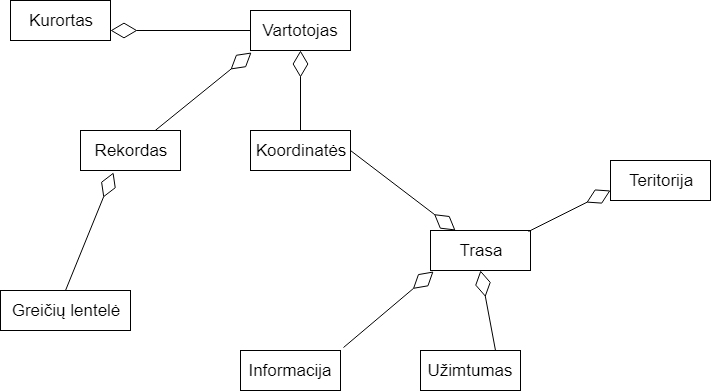
\includegraphics[width=1\textwidth]{DomainModel.png}
    \caption{Domain model diagrama}
    \label{fig:DomainModel}
\end{figure}
\pagebreak

\subsection{Reikalavimų/esybių atsekamumo matrica}	
\begin{figure}[h]
    \centering
    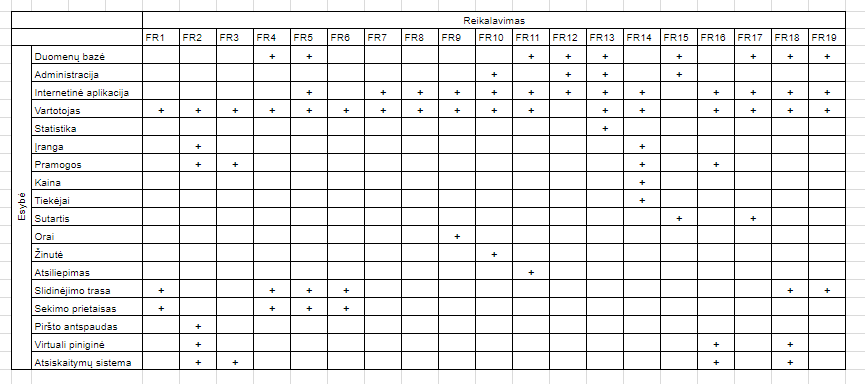
\includegraphics[width=1\textwidth]{Reikalavimai_Esybes.png}
    \caption{Reikalavimų/Esybių atekamumo matrica}
    \label{fig:r/e_matrica}
\end{figure}
\section{Užduotys}
\subsection{Use case diagramos}
\begin{figure}[h]
    \centering
    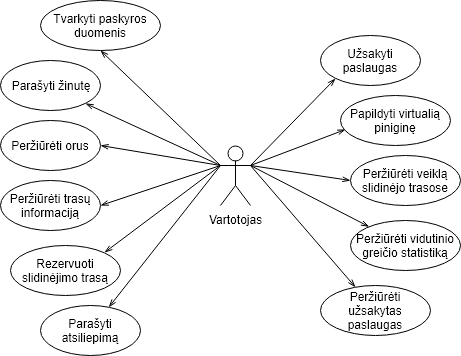
\includegraphics[width=0.75\textwidth]{useCaseVartotojas.png}
    \caption{Vartotojo užduočių diagrama}
    \label{fig:VartotojoUseCasel}
\end{figure}
\vskip 1cm
\begin{figure}[h]
    \centering
    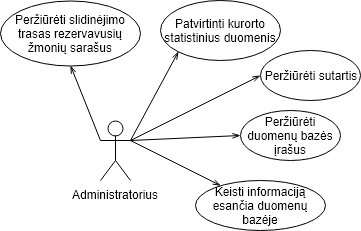
\includegraphics[width=0.65\textwidth]{useCaseAdministratorius.png}
    \caption{Administratoriaus užduočių diagrama}
    \label{fig:AdministratoriausUseCase}
\end{figure}

\begin{figure}[h]
    \centering
    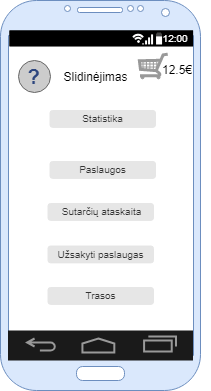
\includegraphics[width=0.30\textwidth]{mainmenu.png}
    \caption{Pagrindinio meniu langas}
    \label{fig:mainmenu}
\end{figure}

\subsection{Vartotojas įsideda pinigų į virtualią piniginę}
Trigeris: Vartotojas aplikacijoje paspaudžia ant pinigų likučio ir atsidariusiame lange paspaudžia "Papildyti piniginę". \\ \\ 
Aktoriai: Vartotojas, administratorius. \\ \\
Pagrindinis scenarijus: Vartotojui pasirinkus "Papildyti sąskaitą" atsidaro langas "Mokėjimo pasirinkimas", kuriame vartotojas gali pasirinkti, kokiu būdu nori papildyti sąskaitą, bei norimą sumą(min 3€). Mokant top-up apmokėjimo būdu vartotojas nukreipiamas į šios paslaugos teikėjo puslapį, o pasirinkus pervedimą vartotojui tame pačiame lange parodoma mokėjimo informacija, naudojantis šiuo būdu pervesti pinigai virtualioje piniginėje atsiranda administratoriui patvirtinus banko pavedimą. Viską atlikęs vartotojas gali pasinaudoti lango apačioje esančiu mygtuku "Grįžti" ir patekti atgal į pagrindinį meniu. \\ \\
Alternatyvūs scenarijai: \\ \\ 
1. Vartotojas atlieka visus nurodytus žingsnius, papildymą atlikdamas bankinio pervedimo būdu, tačiau po 3 darbo dienų jo virtuali piniginė dar nepasipildė, tuo atveju   vartotojas spaudžia klaustuka aplikacijos pagrindiniame lange, jį paspaudus atsidaro langas "Pagalba", kuriame jis nusiunčia atitinkamą pranešimą, prisegdamas pavedimo išrašo kopiją, jam kuo skubiau atrašo administratorius. \\ \\
2. Vartotojas atlieka visus nurodytus žingsnius, papildymą atlikdamas top-up būdu, tačiau mokėjimo metu dingsta prieeiga prie interneto, tuo atveju tas papildymo procesas atšaukiamas ir vartotojui kitą kartą prisijungus tenka visą procesą pradėti nuo pradžių. \\ \\
\begin{figure}[h]
    \centering
    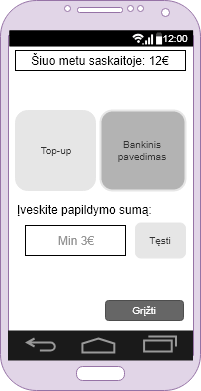
\includegraphics[width=0.20\textwidth]{Mokejimo_Pasirinkimas.png}
    \caption{Mokėjimo pasirinkimo langas}
    \label{fig:apmokejimas}
\end{figure}
\subsection{Vartotojas peržiūri savo mėnesio veiklą slidinėjimo trasose}
Trigeris: Vartotojas aplikacijoje paspaudžia mygtuką "Statistika", atsidaro langas "Vartotojo statistika" jame vartotojas pasirenka mygtuką "Mano trasų istorija" \\ \\
Aktoriai: Vartotojas \\ \\
Pagrindinis scenarijus: Vartotojas paspaudžia mygtuką "Mano trasų istorija", atsidaro langas "Vartotojo istorija", šiame lange vartotojui tinklelio pavidalu(Po du eskizus horizontaliai) pavaizduotos trasos(su pavadinimais), kuriose vartotojas lankėsi per paskutinias 30 dienų, jam paspaudus ant norimos trasos iššoka pop-up langas, kuriame išrašyta vartotojo vidutinis greitis, greičiausias laikas, bei visas praleistas laikas toje trasoje. Susipažinęs su informacija vartotojas spaudžia mygtuką "Gerai", taip pašalindamas pop-up langą ir sugrįždamas į  langą "Vartotojo istorija", kurio apačioje yra mygtukas suteikiantis galimybę grįžti į pagrindinį meniu. \\ \\
Alternatyvūs scenarijai: \\ \\
1. Vartotojas paspaudžia mygtuką "Mano trasų istorija", tačiau per pastarąjį mėnesi jis nebuvo jokioje trasoje, sistema jam parodo atitinkamą pranešimą ir nukreipia atgal į pagrindinį aplikacijos langą. \\
2. Vartotojas paspaudžia mygtuką "Mano trasų istorija", tačiau tuo metu neturi prisijungimo prie interneto, tuo atveju išvedamas pranešimas, kad norint pamatyti šią informaciją reikalingas interneto ryšys. Vartotojas nukreipiamas į pagrindinį meniu. \\
\subsection{Vartotojas peržiūri vidutinį greitį pasirinktoje trasoje}
Trigeris: Vartotojas aplikacijoje paspaudžia mygtuką "Statiska" atsidaro langas "Vartotojo statistika" jame vartotojas pasirenka "Vidutinis greitis" mygtuką. \\ \\
Aktoriai: Vartotojas. \\ \\ 
Pagrindinis scenarijus: Vartotojui pasirinkus, mygtuką "Vidutinis greitis", atsidaro langas "Vidutiniai greičiai", kuriame vartotojas įveda norimos trasos pavadinimą(įvedus 3 pirmas raides sistema pasiūlo galimai tinkamus variantus), bei laikotarpį, kurio vidutinį greitį nori peržiūrėti, bei spaudžia mygtuką "Peržiūrėti". Vartotojui parodoma lentelė, kurioje surašyti kitų vartotojų vid. laikai toje trasoje, bei paryškintai rodomas vartotojo vidutinis laikas, bei šalia šios lentelės parodomas paprastas pasirinktos trasos eskizas. Lango apačioje, dešiniajame kampe vartotojas gali paspausti mygtuką "Grįžti" norėdamas patekti atgal į pagrindinį meniu. \\ \\
Alternatyvūs scenarijai \\ \\
1. Vartotojas veda trasos pavadinimą, tačiau tokia trasa kurorte neegzistuoja, tuo atvėju vartotojui pranešame, kad tokios trasos rasti nepavyko, bei pasiūloma pasitikslinti trąsos pavadinimą, bei bandyti dar kartą. \\ \\
2. Vartotojas suveda trasos pavadinima, bei norimą laikotarpį, tačiau patikrinus aptinkama, kad šiuo laikotarpiu vartotojas joje nebuvo. Tuo atvėju jam parodomas atitinkamas pranešimas ir į ekraną išvedama lentelė, kurioje yra surašyti kitų vartotojų vidutiniai laikai. Vartotojas gali grįžti į pagrindinį meniu paspaudęs mygtuką "Grįžti" esantį lango apačioje, dešinėje pusėje. \\ \\
\begin{figure}[h]
\centering
\parbox{5cm}{
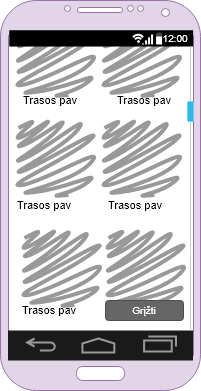
\includegraphics[width=4cm]{ManoTrasuIstorija.png}
\caption{Vartotojo trasu istorija}
\label{fig:2figsA}}
\qquad
\begin{minipage}{5cm}
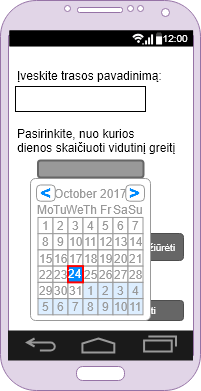
\includegraphics[width=4cm]{VidutiniaiGreičiai.png}
\caption{Vidutiniai greičiai}
\label{fig:2figsB}
\end{minipage}
\end{figure}


\subsection{Paslaugų peržiūra}
	Triggeris: Vartotojas aplikacijoje paspaudžia mygtuką ,,Paslaugos"\\ \\
	Aktoriai: vartotojas\\ \\
	Pagrindinis scenarijus: Vartotojas internetinėje aplikacijoje pasirenka peržiūrėti paslaugas. Sistema vartotoja nukelią į kitą aplikacijos langą kuriame vartotojui suteikiamas pasirinkimas peržiūrėti paslaugas arba kurorte naudojama techniką. Tiek paslaugos tiek technika pateikiama sąrašu, prie kiekvieno sąrašo elemento yra paveiksliukas atitinkanti konkrečia paslaugą ir paslaugos ar įrangos pavadinimas. Vartotojas gali paspausti ant kiekvieno sąrašo elemento sužinoti detalesnią informaciją\\ \\
Alternatyvūs scenarijai:\\ \\
1. Sistema negali pateikti paslaugų sąrašo. Vartotojui parodomas infoirmacinis pranešimas, kad vyksta techniniai darbai ir pasiūloma sugrįšti vėliau. Vartotojui suteikiama galimybė grįšti į pagrindinį aplikacijos langą.\\
2. Nėra detalesnės informacijos apie paslaugą arba įrangą. Vartotojui parašoma, kad papildomos informacijos nėra ir pasiųloma susisiekti su klientų aptarnavimo skyriumi dėl detalesnės informacijos. Vartotojui parodomas aptarnavimo skyriaus elektroninis paštas ir suteikiama galimybė grįšti į pagrindinį aplikacijos langą.

\subsection{Administratorius peržiūri sutarčių ataskaita}
	Triggeris: Administratorius aplikacijos suteiktoje darbo aplinkoje paspaudžia mygtuką ,,Sutarčių ataskaitos"\\ \\
	Aktoriai: administratorius \\ \\
	Pagrindinis scenarijus: Administratorius darbo aplinkoje pasirenka peržiūrėti sutarčių ataskaitas. Sistema iš duombazės gauna ir pateikia sutarčių sąrašą. Kiekvienas sarašo elementas turi pavadinimą, sutarties numerį ir pasirašymo datą. Administratoriui suteikiama galimybė paspaudus ant individualaus sąrašo elemento matyti detalią konkrečios sutarties ataskaitą. Taip pat suteikiama galimybė ieškoti sutarties pagal jos numerį bei rušiuoti sutartis pagal datą \\ \\
	Alternatyvūs scenarijai: \\ \\
1. Administratoriui pasirinkus sutarčių peržiūrą sistemai nepavyksta susisiekti su duomenų baze. Administratoriui pateikiamas klaidfos kodas, serverių statusas, nurodymai kas padėtų išspręsti problemą ir suteikiami techninės pagalbos kontaktai. \\ 
2. Administratorius į paieškos lauką įveda sutarties numerį tačiau tokia sutartis sistemoje neegzistuoja. Prodomas informacinis pranešimas, kad tokia sutartis neegzistuoja \\ \\

\subsection{Vartotojas užsako paslaugas}
	Triggeris: Vartotojas aplikacijoje paspaudžia mygtuką ,,užsakyti paslaugas" \\ \\
	Aktoriai: vartotojas \\ \\
	Pagrindinis scenarijus: Vartotojas internetinėje aplikacijoje paspaudžia mygtuką ,,Užsisakyti paslaugas". Vartotojui pateikiamas paslaugų sąraša ir kiekvienos paslaugos kaina vienam žmogui. Vartotojas turi galimybę pasirinkti paslaugą užsakyti ją iki 10 žmonių ir pasirinkti paslaugos laiką. Varotojui parašius žmonių skaičių ir patvirtinus užsakymą jis atsiranda prekių krepšelyje ir paslaugos kaina pridedama prie bendros krepšelio kainos. \\ \\
	Alternatyvūs scenarijai:  \\ \\
1. Vartotojui pasirinkus užsakyti konkrečia paslaugą ir jos laiką ši paslauga tuo laiku negalima. Vartotojui parodomas pranešimas, kad paslauga tuo metu negalima. Vartotojui pateikiamas artimiausias laisvas laikas. \\ 
2. Vartotojui pasirinkus užsakyti paslaugą sistema negali nusiųsti paslaugos užsakymo užklausos. Vartotojui parodomas informacinis pranešimas kad vyksta techniniai darbai ir paslaugų užsakyti negalima. Vartotojui paskiūloma paslaugą užsisakyti telefonu paskambinus į kurortą, užsakymą parašyti elektroniniu paštu arba sugrįšti vėliau.\\ \\

\subsection{Vartotojas peržiūri užsakytas paslaugas}
	Trigeris: Vartotojas aplikacijoje paspaudžia mygtuką ,,Paslaugos"\\ \\
	Aktoriai: Vartotojas\\ \\
	Pagrindinis scenarijus: Vartotojas internetinėje aplikacijoje paspaudžia mygtuką ,,Paslaugos". Vartotojui pateikiamas jo užsakytų paslaugų sąrašas. Vartotojui suteikiama galimybė paspaudus ant individualaus sąrašo elemento matyti detalią paslaugos informaciją.\\ \\
	Alternatyvūs scenarijai:\\ \\
1. Vartotojui pasirinkus užsakytų paslaugų peržiūrą nerandama užsakytų paslaugų. Vartotojui parodoma nuoroda užsakyti paslaugas. Vartotojui siūloma palaukti, jei neseniai užsisakė paslaugą. Vartotojui siūloma kreiptis pagalbos, jei nuo paslaugos užsakymo jau praėjo diena laiko.\\ \\
2. Vartotojui pasirinkus užsakytų paslaugų peržiūrą sistema negali susisiekti su duomenų baze. Vartotojui parodomas pranešimas, kad vyksta techniniai darbai ir pasiūloma sugrįšti vėliau. Vartotojui pateikiama nuoroda grįšti į pagrindinį puslapį.\\ \\

\begin{figure}[h]
\centering
\parbox{5cm}{
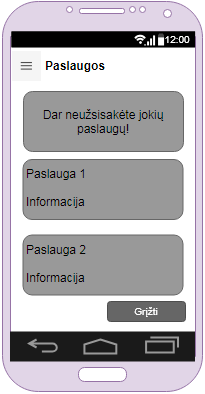
\includegraphics[width=4cm]{GUI-17-uzsakytos-paslaugos(1).png}
\caption{Vartotojas neužsisakė jokių paslaugų}
\label{fig:2figsA}}
\qquad
\begin{minipage}{5cm}
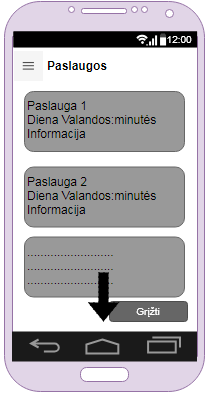
\includegraphics[width=4cm]{GUI-17-uzsakytos-paslaugos(2).png}
\caption{Paslaugos ir jų užsakymo laikas}
\label{fig:2figsB}
\end{minipage}
\begin{minipage}{5cm}
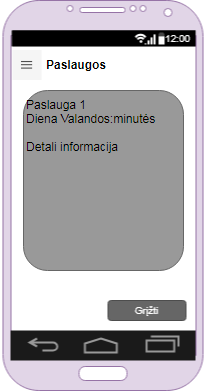
\includegraphics[width=4cm]{GUI-17-uzsakytos-paslaugos(3).png}
\caption{Detali paslaugos informacija}
\label{fig:2figsC}
\end{minipage}
\end{figure}


\subsection{Vartotojas rezervuoja trasą}
	Trigeris: Vartotojas aplikacijoje paspaudžia mygtuką ,,Trasos"\\ \\
	Aktoriai: Vartotojas\\ \\
	Pagrindinis scenarijus: Vartotojas internetinėje aplikacijoje paspaudžia mygtuką ,,Trasos". Vartotojui pateikiamas trasų sąrašas. Vartotojui suteikiama galimybė paspaudus ant individualaus sąrašo elemento matyti detalią trasos informaciją ir laisvas rezervacijai dienas bei valandas. Vartotojui pasirinkus laiką ir patvirtinus užsakymą, užsakymas pridedamas į krepšelį. Vartotojui parodomas pranešimas apie sėkmingai pridėtą užsakymą ir pasiūloma peržiūrėti prekių krepšelį.\\ \\
	Alternatyvūs scenarijai:\\ \\
1. Vartotojui besirenkant rezervacijos laiką įvyksta kitas užsakymas ir jo pasirinktas laikas tampa užimtas. Vartotojui patvirtinus užsakymą parodomas pranešimas, kad trasa tuo laiku užimta. Vartotojui pasiūloma atnaujinti langą ir pamatyti naują trasos užimtumą.\\ \\
2. Vartotojui paspaudus mygtuką ,,Trasos" trasų sąrašas yra tuščias. Vartotojui siūloma dėl trasų rezervacijos pasiteirauti telefonu ar elektroniniu paštu.\\ \\
3. Vartotojui paspaudus mygtuką ,,Trasos" sistema negali susisiekti su duomenų baze. Vartotojui parodomas pranešimas, kad vyksta techniniai darbai ir pasiūloma sugrįšti vėliau. Vartotojui pateikiama nuoroda grįšti į pagrindinį puslapį.\\ \\

\begin{figure}[h]
\centering
\parbox{5cm}{
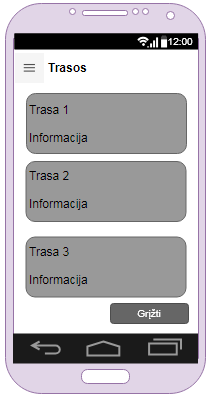
\includegraphics[width=4cm]{GUI-18-19-trasos.png}
\caption{Visos trasos}
\label{fig:2figsA}}
\qquad
\begin{minipage}{5cm}
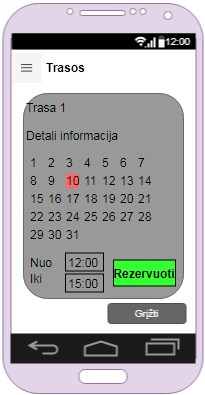
\includegraphics[width=4cm]{GUI-18-19-detali-trasos-informacija.png}
\caption{Rezervuoti trasą}
\label{fig:2figsB}
\end{minipage}
\end{figure}

\subsection{Vartotojas peržiūri informaciją apie trasą}
	Trigeris: Vartotojas aplikacijoje paspaudžia mygtuką ,,Trasos"\\ \\
	Aktoriai: Vartotojas\\ \\
	Pagrindinis scenarijus: Vartotojas internetinėje aplikacijoje paspaudžia mygtuką ,,Trasos". Vartotojui pateikiamas trasų sąrašas. Vartotojui paspaudus ant individualaus sąrašo elemento parodoma detalesnė trasos informacija.\\ \\
	Alternatyvūs scenarijai:\\ \\
1. Vartotojui paspaudus ant sąrašo elemento trūksta informacijos apie trasą. Vartotojui pasiūloma pasiteirauti telefonu ar elektroniniu paštu.\\ \\
2. Vartotojui paspaudus mygtuką ,,Trasos" sistema negali susisiekti su duomenų baze. Vartotojui parodomas pranešimas, kad vyksta techniniai darbai ir pasiūloma sugrįšti vėliau. Vartotojui pateikiama nuoroda grįšti į pagrindinį puslapį.\\ \\
	
\subsection{Vartotojas peržiūri orus}
	Triggeris: Vartotojas aplikacijoje paspaudžia mygtuką "Orai", atsidaro naujas langas "Orų peržiūra" \\ \\
	Aktoriai: Vartotojas \\ \\
	Pagrindinis scenarijus: Vartotojas aplikacijoje paspaudžia mygtuką "Orai". Atidaromas naujas langas "Orų peržiūra", kuriame yra du mygtukai: "Dabartiniai orai" ir "Orų prognozė". Vartotojas paspaudžia mygtuką "Dabartiniai orai" ir aplikacijoje atsidaro langas kuriame rodoma dabartinė temperatūra, drėgmė, krituliai bei vėjo greitis. Peržiūrėjęs orus vartotojas uždaro langą paspausdamas mygtuką "Grįžti į pagrindinį meniu". \\
	Alternatyvus scenarijus: Vartotojas paspaudžia mygtuka "Orai". Atidaromas naujas langas "Orų peržiūra", tačiau nepavyksta prisijungti prie orų sekimo įrenginio. Vartotojui parodomas pranešimas, jog nepavyko prisijungti prie orų sekiklio ir prašoma pabandyti vėliau. Vartotojas gražinamas į pagrindinį meniu. \\ \\

\begin{figure}[h]
    \centering
    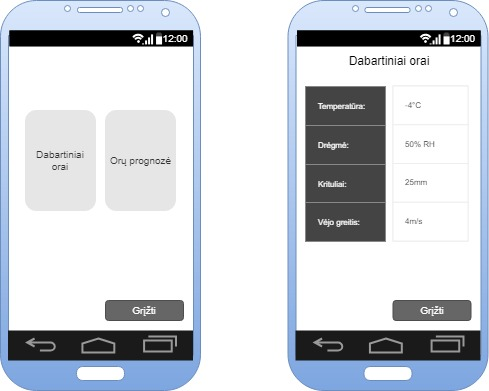
\includegraphics[width=0.80\textwidth]{GUI11.jpg}
    \caption{Orų peržiūros langas}
    \label{fig:orai}
\end{figure}


\subsection{Vartotojas rašo žinutę}
	Triggeris: Vartotojas aplikacijoje paspaudžia mygtuką "Rašyti naują žinutę", jam iššoka langas "Nauja žinutė" \\ \\
	Aktoriai: Vartotojas \\ \\
	Pagrindinis scenarijus: Vartotojas aplikacijoje paspaudžia mygtuką "Rašyti naują žinutę", jam iššoka langas "Nauja žinutė". Vartotojas pasirenka gavėją (kitas vartotojas, administratorius ar maisto į kamabarį tarnyba), nurodo gavėjo vardą (jei to reikia), nurodo žinutės temą, parašo žinutę ir ją išsiunčia paspausdamas mygtuką "Siųsti žinutę". Išsiuntus žinutę vartotojui atidaromas naujas langas "Nauja žinutė", kurį jis uždaro paspausdamas mygtuką "Atgal". \\ \\
	Alternatyvus scenarijus: Vartotojas aplikacijoje paspaudžia mygtuką "Rašyti naują žinutę", jam iššoka langas "Nauja žinutė". Vartotojas pasirenka gavėją (kitas vartotojas, administratorius ar maisto į kamabarį tarnyba), nurodo gavėjo vardą (jei to reikia), nurodo žinutės temą, parašo žinutę ir ją išsiunčia paspausdamas mygtuką "Siųsti žinutę", tačiau neteisingai nurodo gavėjo vardą ir žinutė neišsiunčiama. Sistema vartotojui išmeta klaidos pranešimą ir leidžia jam atlikti norimus pakeitimus. \\ \\

\subsection{Vartotojas parašo atsiliepimą}
	Triggeris: Vartotojas aplikacijoje paspaudžia mygtuką "Rašyti atsiliepimą", atsidaro naujas langas "Atsiliepimai" \\ \\
	Aktoriai: Vartotojas \\ \\
	Pagrindinis scenarijus: Vartotojas paspaudžia mygtuką "Rašyti atsiliepimą". Aplikacijoje atsidaro naujas langas "Atsiliepimai", kuriame vartotojas gali sukurti naują atsiliepimą. Vartotojas įvertina savo viešnagę 1-5 žvaigždutėm, bei atskirame laukelyje parašo savo komentarus. Baigęs rašyti savo atsiliepimą vartotojas paspaudžia mygtuką "Siųsti" ir atsiliepimas išsiunčiamas. Vartotojas paspaudžia mygtuką atgal ir grįžta į pagrindinį meniu. \\ \\
	Alternatyvus scenarijus: Vartotojas paspaudžia mygtuką "Rašyti atsiliepimą". Aplikacijoje atsidaro naujas langas "Atsiliepimai", kuriame vartotojas gali sukurti naują atsiliepimą. Vartotojas laukelyje parašo komentarus apie savo viešnagę. Baigęs rašyti savo atsiliepimą vartotojas paspaudžia mygtuką "Siųsti", tačiau vartotojas neįvertino savo viešnagės. Vartotojo paprašoma pateikti 1-5 žvaigždučių įvertinimą. Vartotojas baigęs grįžta į pagrindinį meniu paspaudęs mygtuką "Atgal". \\ \\

\begin{figure}[h]
    \centering
    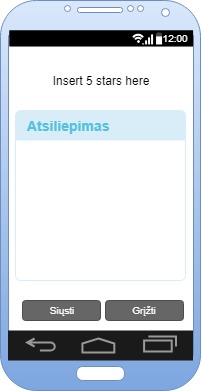
\includegraphics[width=0.30\textwidth]{GUI13.jpg}
    \caption{Atsiliepimo parašymo langas}
    \label{fig:atsiliepimas}
\end{figure}


\subsection{Administratorius peržiūri duomenų bazę}
	Triggeris: Administratorius aplikacijoje paspaudžia mygtuką "Peržiūrėti duomenų bazę", jam atidaromas duombazės peržiūros langas "Duomenų bazės peržiūra"
	Aktoriai: Administratorius
	Pagrindinis scenarijus: Administratorius paspaudžia mygtuką "Peržiūrėti duomenų bazę", jam prisijungiama prie duomanų bazės ir atidaromas duombazės peržiūros langas "Duomenų bazės peržiūra". Administratorius stebi duomenų bazėje esančių objektų būseną. Administratorius pasirenka objektą ir pakeičia jo duomenis. Padaręs pakeitimus, administratorius juo išsaugo paspaudęs mygtuką "Saugoti" ir baigęs darbą su duombaze, nuo jos atsijungia paspausdamas mygtuką "Atgal". \\ \\
	Alternatyvūs scenarijai:  \\ \\ 
1. Administratorius paspaudžia mygtuką "Peržiūrėti duomenų bazę", tačiau sistemai nepavyksta prisijungti prie duomenų bazės. Administratoriui išmetamas pranešimas, jog nepavyko prisijungti prie duomenų bazės ir paprašoma jo bandyti vėliau. Administratorius grąžinamas į pagrindinį meniu. \\
2. Administratorius paspaudžia mygtuką "Peržiūrėti duomenų bazę", jam prisijungiama prie duomanų bazės ir atidaromas duombazės peržiūros langas "Duomenų bazės peržiūra". Administratorius stebi duomenų bazėje esančių objektų būseną. Administratorius pasirenka objektą ir pakeičia jo duomenis. Padaręs pakeitimus administratorius bando atsijungti nuo duomenų bazės spausdamas mygtuką "Atgal". Sistema išmeta pranšimą, jog jo padaryti pakeitimai nėra išsaugoti ir paklausia ar jis nori išsaugoti pakeitimus. Administratorius paspaudžia mygtuką "Taip", tada paspaudžia mygtuką "Saugoti" ir atsijungia nuo duomenų bazės paspausdamas mygtuką "Atgal", kuris grąžina jį į pagrindinį meniu. \\ \\

\subsection{Vartotojas pepržiūri savo poziciją ir laiką praleistą trasoje}
Triggeris: Vartotojas paspaudžia mygtuką ''Žemėlapis''.\\ \\
Aktoriai: vartotojas.\\ \\
Pagrindinis scenarijus: Vartotojas paspaudžia mygtuką ''Žemėlapis'', atsiveria langas su trasų žemėlapiu. Raudonu tašku pažymėta vartotojo dabartinė vieta. Apačioje rodomas trasos pavadinimas, praleistas ir likęs vartotojo laikas joje. Paspaudus ant trasų pavadinimo žemėlapyje atveriamas langas su detalesne informacija apie ją.\\ \\
Alternatyvūs scenarijai:  \\ \\
1. Vartotojas paspaudžia mygtuką ''Žemėlapis'', atveriamas langas su trasų žemėlapiu, bet nerandama vartotojo dabartinė vieta. Vartotojui parodomas langas, kuriame siūloma įsijungti GPS, o alternatyviai - pagalbos telefonas.\\
2. Vartotojas paspaudžia mygtuką ''Žemėlapis'', atveriamas langas su trasų žemėlapiu. Paspaudus ant trasos pavadinimo, atveriamas naujas langas, bet trūksta informacijos jame.  Vartotojui pasiūloma pasiteirauti telefonu ar elektroniniu paštu. \\ \\ 

\subsection{Vartotojas nori pasikeisti asmeninis duomenis}
Triggeris: Vartotojas paspaudžia mygtuką ''Profilis''. \\ \\
Aktoriai: Vartotojas.\\ \\
Pagrindinis scenarijus: Vartotojas paspaudžia mygtuką ''Profilis'', jam atveriamas langas su laukais: Vardas, Pavardė, El. paštas, Keisti slaptažodį. Galima redaguoti visus laukus. Paspaudus 'Keisti slaptažodį'' sugeneruojamas naujas raktas ir jis išsiunčiamas į jo el. paštą. Apačioje yra mygtukas ''Atsijungti''. Jį paspaudus vartotojas atjungiamas nuo sistemos ir jam atveriamas prisijungimo langas. \\ \\
Alternatyvus scenarijus: Vartotojas paspaudžia mygtuką ''Profilis'', jam atveriamas langas su laukais: Vardas, Pavardė, El. paštas, Keisti slaptažodį.  Paspaudus ''Keisti slaptažodį'' sugeneruojamas naujas raktas ir pranešama, kad slaptažodis išsiųstas į nurodytą el. paštą. Vartotojui jo negavus, spaudžiamas mygtukas ''Siųsti iš naujo''. Išvedamas pranešimas, kad slaptažodis išsiųstas ir pasiūloma pasitikrinti  ''Spam'' folderį. \\ \\ 

\subsection{Reikalavimų - užduočių atsekamumo matrica}
\begin{figure}[h]
    \centering
    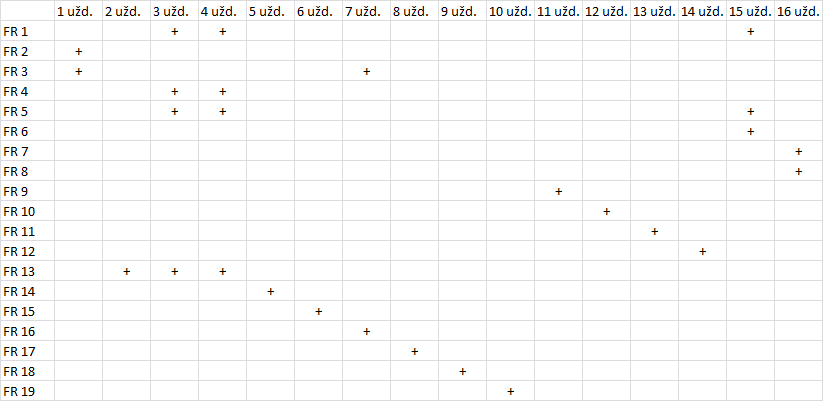
\includegraphics[width=1\textwidth]{reik_uzd_matrica_before.png}
    \caption{Reikalavimų/Užduočių atsekamumo matrica}
    \label{fig:matrica}
\end{figure}

\section{Reikalavimų specifikacijos, dalykinės srities modelio ir užduočių diagramos peržiūros rezultatai}
\subsection{Reikalavimų specifikacijos peržiūra}
\subsubsection{Funkcinių reikalavimų specifikacijos pokyčių lentelė}
\begin{longtable}{ | p{0.1\textwidth}|p{0.20\textwidth}|p{0.09\textwidth}|p{0.15\textwidth}|p{0.40\textwidth}| }  \hline
	Pataisymo nr. & Pradiniai reikalavimas &  Pakeitimo tipas & Klaidos aprašas  & Naujas reikalavimas \\ \hline
	0. & FR 2: Sistema suteikia vartotojui įsidėti pinigų į virtualią piniginę. Atsiskaitinėjant vartotojas gali būti intentifikuojamas piršto antspaudu & M & 2 reikalavimai sudėti į vieną 
	& FR 2. Sistema suteikia vartotojui įsidėti pinigų į virtualią piniginę. \newline
	2.1 Top-up metodu. \newline
	2.2 Pervedimo būdu. \newline \newline
	FR 3. Atsiskaitinėjant vartotojas gali identifikuotis piršto antspaudu. \\ \hline

	1. & FR 7: Sistema suteikia vartotojui galimybę pakeisti savo asmeninius duomenis ir atsijunti nuo paskyros \newline
		 FR 8: Sistema suteikia vartotojui galimybę atnaujinti savo paskyros slaptažodį & M & Susiję reikalavimai užrašyti atskirai 	 
	& FR 7. Sistema vartotojui suteikia galimybę tvarkyti savo paskyrą \newline
	7.1 Prisijungti \newline
	7.2 Atsijungti \newline
	7.3 Keisti asmeninius duomenis \newline
	7.4 Keisti paskyros slaptažodį \\ \hline

	2. & FR 12: Internetinė aplikacija administratoriui suteikia galimybę stebėti duombazės objektų būseną ir ją keisti & M & Reikalavimas abstraktus, nepakankamai aiškus 
	& FR 13. Internetinė aplikacija administratoriui suteikia galimybę tvarkyti duomenis esančius duomenų bazėje \newline
	13.1    Tvarkyti trasų duomenis. \newline
	13.2    Tvarkyti kurorto statistinius duomenis. \newline
	13.3    Tvarkyti atsiliepimus. \\ \hline

	3. & FR 13: Internetinė aplikacija, duombazės pagalba, suteikia vartotojui galimybę peržiūrėti kurorto ir vartotojo statistiką. Rodomi statistiniai duomenys turi būti patvirtinti administracijos ir kurorto vadovo. & M & Reikalavimas netikslus
	& FR 14. Internetinė aplikacija suteikia vartotojui galimybę statistiką.  \newline
	14.1    Vartotojas turi galėti peržiūrėti savo statistiką \newline
	14.2    Vartotojas turi galėti peržiūrėti kurorto statistiką, jeigu ji patvirtinta administratoriaus \newline
	14.2.1		Administratorius turi galėti patvirtinti arba atmesti naują statistiką apie kurortą \\ \hline

	4. & FR 16: Sistema per aplikacija vartotojui suteikia galimybę užsisakyti paslaugas & M & Per daug abstraktus reikalavimas 
	& FR 17. Sistema per aplikacija vartotojui suteikia galimybę užsisakyti paslaugas \newline
	17.1	Užsisakyti maisto į viešbučio kambarį \newline
	17.2	Rezervuoti slidinėjimo įrangą \\ \hline

	5. & FR 1: Sistema seka vartotojų laiką praleista trasoje pasinaudodama sekimo prietaisu & M & Pakeistas reikalavimas, ištrintas nefunkcinis reikalavimo elementas & FR 1:  Sistema seka vartotoją trasoje, rodo jo poziciją ir praleistą laiką trasoje\\ \hline
	
	6. & FR 6: Sistema seka kiekvieno vartojo laiką praleistą trasoje ir poziciją jam esant kurorte. & X & Reikalavimas dubliuojasi su FR 1 & -\\ \hline


\end{longtable}

\subsubsection{Pataisyta funkcinių reikalavimų specifikacija}
\begin{enumerate}
	\item Sistema seka vartotojų laiką praleista trasoje pasinaudodama sekimo prietaisu.
	\item Sistema suteikia vartotojui įsidėti pinigų į virtualią piniginę.
	\begin{enumerate}
		\item Top-up metodu.
		\item Pervedimo būdu.
	\end{enumerate}
	\item Atsiskaitinėjant vartotojas gali identifikuotis piršto antspaudu.
	\item Sistema leidžia vartotojui už paslaugas atsiskaityti e-bankininkyste.
	\item Sekimo prietaisas fiksuoją greičiausią laiką, per kurį vartotojas įveikė trasą.
	\begin{enumerate}
		\item sistema saugo greičiausią laiką, per kurį vartotojas įveikė trasą.
	\end{enumerate}
	\item Vartotojo trasų laikai rodomi internetinėje aplikacijoje.
	\item Sistema suteikia vartotojui galimybę tvarkyti savo paskyrą.
	\begin{enumerate}
		\item Prisijungti.
		\item Atsijungti.
		\item Keisti asmeninius duomenis.
		\item Keisti paskyros slaptažodį.
	\end{enumerate}
	\item Sistema internetinės aplikacijos pagalba vartotojui suteikia galimybę peržiūrėti orus.
	\begin{enumerate}
		\item Sistema turi pateikti dabartines oro sąlygas.
		\item Sistema turi pateikti ateinančių dienų oru prognozę.
		\begin{enumerate}
			\item temperaturą.
			\item drėgmę.
			\item kritulius.
			\item Vėjo greitį.
		\end{enumerate}
	\end{enumerate}
	\item Internetinėje aplikacijoje vartotojas gali rašyti žinutes kitiems kurorto svečiams, adminisntracijai ir maisto į kambarį tarnybai.
	\item Sistema vartotojui suteikia galimybę rašyti atsiliepimą apie jo viešnagę kurorte ir skirti viešą vertinimą kurortui.
	\begin{enumerate}
		\item Sistema suteikia galimybę keisti vertinimą.
		\item Sistema neleidžia vertinti kurorto kelis kartus tam pačiam asmeniui dažniau, nei kartą per 2 mėnesius.
	\end{enumerate}
	\item Internetinė aplikacija administratoriui suteikia galimybę tvarkyti duomenis esančius duomenų bazėje.
	\begin{enumerate}
		\item Tvarkyti trasų duomenis.
		\item Tvarkyti kurorto statistinius duomenis.
		\item Tvarkyti atsiliepimus.
	\end{enumerate}
	\item Internetinė aplikacija suteikia vartotojui galimybę statistiką.
	\begin{enumerate}
		\item Vartotojas turi galėti peržiūrėti savo statistiką.
		\item Vartotojas turi galėti peržiūrėti kurorto statistiką, jeigu ji patvirtinta administratoriaus.
		\begin{enumerate}
			\item Administratorius turi galėti patvirtinti arba atmesti naują statistiką apie kurortą.
		\end{enumerate}
	\end{enumerate}
	\item Sistemoja per internetinę aplikaciją vartotojui suteikia galimybę peržiūrėti paslaugų kainas, tiekėjų sąrašą ir kiekvienos įrangos technines charakteristikas.
	\item Sistema administratoriui suteikia galimybę skaityti sutarčių ataskaitas.
	\item Sistema per aplikacija vartotojui suteikia galimybę užsisakyti paslaugas.
	\begin{enumerate}
		\item Užsisakyti maisto į viešbučio kambarį.
		\item Rezervuoti slidinėjimo įranga.
	\end{enumerate}
	\item Sistema internetinės aplikacijos pagalba leidžia vartotojui peržiūrėti visas jo pasirašytas sutartis.
	\item Vartotojas turi galimybę užrezervuoti slidinėjimo trasą nurodant: trasos pavadinimą, telefono numerį, slidinėtojų skaičių ir rezervacijos laikotarpį per internetinę aplikaciją.
	\item Vartotojas gali matyti informaciją apie slidinėjimo trasą:pavadinimą,sunkumą, rūšį, nuomos kainą, užimtumą.
	\item \textit{Sistema vartotojui suteikia galimybę peržiūrėti jo užsakytas paslaugas}
	\item \textit{Sistema administratoriui suteikia galimybę pamatysi trasas rezervavusių žmonių sąrašą}
\end{enumerate}

\subsection{Pataisyta nefunkcinių reikalavimų specifikacija}
\begin{enumerate}
	\item Slidinėjimo trasų įrangos bei kambarių pavadinimams maksimaliai skiriama 64 simbolių
	\item Slidinėjimo trasos ilgis vaiduojamas vieno skaičiaus po kablelio tikslumu
	\begin{enumerate}
		\item Ilgio matavimo vienetas - kilometras
	\end{enumerate}
	\item Slidinėjimo trasos statumas vaizduoja vieno skaičio po kablelio tikslumu
	\begin{enumerate}
		\item Statumo matavimo vienetas - procentai
	\end{enumerate}
	\item Slidinėjimo trasų, įrangos bei apgyvendinimo įstaigos laisvų vietų skaičius rodomas vientų tikslumu.
	\item Slidinėjimo trasų, įrangos bei apgyvendinimo įstaigos kainos pateikiamos centų po kablelio tikslumu (10,11eu)
	\item Data turi būti vaizduojama formatu YYYY-MM-DD
	\begin{enumerate}
		\item YYYY - metai
		\item MM - mėnuo
		\item DD - diena
	\end{enumerate}
	\item Laikas turi būti vaizduojamas formatu hh:mm 24 valandų formatu (21:47)
	\begin{enumerate}
		\item hh - valandos. 24 valandų formatu
		\item mm - minutės
	\end{enumerate}
	\item Vartotojo vardui, pavardei, elektroniniam paštui, slaptažodžiui registracijos formoje maksimaliai skiriama 64 simboliai. Taip pat registracijos formoje vartotojams reikia įvesti slaptažodį kuriam maksimaliai skiriama 512 simboliai.
	\item Vartotojo raktas sugeneruojamas pagal GUID
	\item Vartotojo elektroniniam paštui prisijungiant skiriama 64 simboliai o slaptažodžiui 512
	\item Vartotojo slaptažodis negali būti trumpesnis negu 10 simbolių
	\item Vardui, pavardei ir elektroniniam paštui rezervacijos formoje skiriama 64 simboliai
	\item Telefono numeriui rezervacijos formoje skiriama 15 simbolių
	\item Svečių skaičiuo rezervacijos formoje maksimaliai skiriama 3 skaičiai
	\item Orų temperatūra rodoma vienetų tikslumu. Matavimo vienetas celsijus
	\item Rezervacijos/užsakyo/sutarties numeris pateikiamas vienetų tikslumu
	\item Įrangos dydžiai - europietiški. Vaizduojama vienetų tikslumu
	\item Keičiant naršyklės dydį, tinklapio vaizdas pritaikomas automatiškai(Responsive design).
	\item Sistema turi veikti 95proc laiko per dieną. Tai yra leidžiama neveikti 1 valandą 10 min.	
	\item Registruojant naują vartotoją sistema turi patikrinti ar teisingai įvesti jo duomenys.
	\item Prisijungiant vartotojui sistema turi patikrinti ar įvesti duomenys teisingi.
	\item Vartotojui rezervuojant paslaugas sistema turi patikrinti ar duomenys įvesti korektiškai
	\item Vartotojui rezervuoijant paslaugas sistema rezervacijai turi priskirti uniklalų numerį.
	\item Modifikuojama tinklapio atsarginė kopija po kiekvieno informacijos atnaujinimo apie slidinėjimo kurortą, orų prognozes, slidinėjimo trasa, įrangą, apgyvendinimo įstaigą, jų užimtumą bei po kiekvienos esybės registracijos ir įvestos informacijos pakeitimo.
	\item Bandant pildyti laukus ne pagal pateiktus reikalavimus, užklausa negali būti įvykdyta.
	\item Sistemoje turi būti įdiegtos apsaugos priemonės nuo duomenų sugadinimo, praradimo, klaidingų duomenų įvedimo į duomenų bazėje.
	\item Po kiekvienos sėkmingos operacijos pakeitimai turi būti išsaugoti duomenų bazėje.
	\item Nepavykus prisijungti arba negavus duomenų iš duomenų bazės, sistema turi informuoti vartotoją parodydamas klaidos pranešimą
	\item Didžiausia leistina tinklalapio apkrova yra 10000 vartotojų vienu metu
	\item Tinklalapio didžiausia leistinas reakcijos laikas, neįvertinant interneto greičio turi būti ne didesnis kaip 2 sekundės.
	\item Užklausos vykdymo laikas turi būti ne didesnis nei 3 sekundės
	\item Konkrečios slidinėjimo trasos, įrangos, kambario, jų užimtumo paieškai duomenų bazėje turi būti sugaišta ne ilgiau nei 3 sekundės
	\item Tinklapis pasiekiamas prisijungiant iš bet kurio IP adreso
	\item Pradinėje sistemoje turi būti administratoriaus prisijungimo duomenys
	\item Pasirinkimų lentelė turi turėti bent 5 pradines užpildytas eilutes su informacija apie slidinėjimo trasas, įrangą, kambarius. Šią informaciją įveda įgaliotas įmonės administratoriusinterfeisu.
	\item Sistemos turi funkcionuoti lietuvių ir anglų kalbomis
	\item Įmonės darbuotojai turi būti apmokomi naudotis sistema
	\item Tinkalpyje negali būti klaidinančios informacijos
	\item Pakeitimai turi būti įvykdyti ne vėliau nei per 7 darbo dienas po sėkmingo testavimo.
	\item Visi vartotojo atliekami veiksmai turi būti saugomi laikinoje duomenų bazėje, kad atradus klaidą tinklalapyje būtų galima testavimo metu atkurti konkrečia klaidą
	\item Pastebėtos ar esybės praneštos klaidos turi būti ištaisytos kaip galima greičiau.
	\item Į vartotojo atsiųstus laiškus su pastebėjimai ir skundais reikia atsakyti automatine žinute.
	\item Sistema atnaujinti reikia tuo metu, kai yra mažiausias vartotojų srautas
	\item Internetinė aplikacija turi veikti vet kuriame įrenginyje, kuris turi naršyklę palaikančia HTML5 standartą.
	\item Vartotojui prisijungiant prie sistemos vykdoma jo indentifikacija.
	\item Duomenų bazėje saugomas slaptažodžių maišos kodas sumaišytas SHA512 algoritmu.
	\item Visi duomenys apie sistema saugomi duomenų bazėje, o prie jos prieeiga turi tik įgalioti asmenys.
	\item Atsarginė duomenų bazės kopija turi būti daroma reguleriai kas 7 darbo dienas.
	\item Jeigu eisybė neaktyvi ilgiau nei 15 minučių, vartotojas automatiškai atjungiamas.
	\item Kuriant sistemą projekto komandai draudžiama naudotis nelegalia programine įranga
	\item Duomenų perdavimas ir saugojimas neturi pažeisti LR asmens duomenų teisinės apsaugos įstatymo.
	\item Esybių asmeniniai duomenys turi būti įslaptinti t.y. tinklapyje negali būti saugoti ekoduoti duomenys

\end{enumerate}

\subsection{Use case peržiūra}
\subsubsection{Use case pokyčių lentelė}
\begin{longtable}{ | p{0.2\textwidth}|p{0.2\textwidth}|p{0.5\textwidth}| }  \hline
	Pataisymo nr. & Use case numeris & Klaidos aprašas \\ \hline
	0 & 5 & Use case aprašyme nėra paminėti visi naudojami GUI komponentai \\ \hline
	1 & 6 & Use case aprašyme nėra paminėti visi naudojami GUI komponentai \\ \hline
	2 & 7 & Use case aprašyme nėra paminėti visi naudojami GUI komponentai \\ \hline
	3 & 8 & Use case aprašyme nėra paminėti visi naudojami GUI komponentai \\ \hline
	4 & 9 & Use case aprašyme nėra paminėti visi naudojami GUI komponentai \\ \hline
	5 & 10 & Use case aprašyme nėra paminėti visi naudojami GUI komponentai \\ \hline
	6 & 15 & Use case aprašyme nėra paminėti visi naudojami GUI komponentai \\ \hline
	7 & 16 & Use case aprašyme nėra paminėti visi naudojami GUI komponentai \\ \hline
\end{longtable}

\subsubsection{Pataisyti use case}

\subsubsubsection{}
	Triggeris: Vartotojas aplikacijoje paspaudžia mygtuką "Paslaugos" ir jam atidaromas langas "Paslaugų peržiūra"
	Pagrindis scenarijus: Vartotojas internetinėje aplikacijoje pasirenka peržiūrėti paslaugas. Sistema vartotoja nukelią į kitą aplikacijos langą "Paslaugų peržiūra" kuriame vartotojui suteikiamas pasirinkimas peržiūrėti paslaugas arba kurorte naudojama techniką. Tiek paslaugos tiek technika pateikiama sąrašu, prie kiekvieno sąrašo elemento yra paveiksliukas atitinkanti konkrečia paslaugą ir paslaugos ar įrangos pavadinimas. Vartotojas gali paspausti ant kiekvieno sąrašo elemento sužinoti detalesnią informaciją
\subsubsubsection{}
	Triggeris: Administratorius aplikacijos suteiktoje darbo aplinkoje paspaudžia mygtuką "Sutarčių ataskaitos" ir jam atidaromas langas "Ataskaitos"
	Pagrindinis scenarijus: Administratorius darbo aplinkoje pasirenka peržiūrėti sutarčių ataskaitas. Sistema iš duombazės gauna ir atvaizduoja sutarčių sąrašą lange "Ataskaitos". Kiekvienas sarašo elementas turi pavadinimą, sutarties numerį ir pasirašymo datą. Administratoriui suteikiama galimybė paspaudus ant individualaus sąrašo elemento matyti detalią konkrečios sutarties ataskaitą. Taip pat suteikiama galimybė ieškoti sutarties pagal jos numerį bei rušiuoti sutartis pagal datą
\subsubsubsection{}
	Triggeris: Vartotojas aplikacijoje paspaudžia mygtuką "užsakyti paslaugas", atidaromas langas "Paslaugos užsakymas"
	Pagrindinis scenarijus: Vartotojas internetinėje aplikacijoje paspaudžia mygtuką "Užsisakyti paslaugas". Vartotojui pateikiamas paslaugų sąrašas lange "Paslaugos užsakymas" ir kiekvienos paslaugos kaina vienam žmogui. Vartotojas turi galimybę pasirinkti paslaugą užsakyti ją iki 10 žmonių ir pasirinkti paslaugos laiką. Varotojui parašius žmonių skaičių ir patvirtinus užsakymą jis atsiranda prekių krepšelyje ir paslaugos kaina pridedama prie bendros krepšelio kainos.
\subsubsubsection{}
	Trigeris: Vartotojas aplikacijoje paspaudžia mygtuką "Paslaugos", atidaromas langas "Palaugos"
	Pagrindinis scenarijus: Vartotojas internetinėje aplikacijoje paspaudžia mygtuką "Paslaugos". Vartotojui pateikiamas jo užsakytų paslaugų sąrašas lange "Paslaugos". Vartotojui suteikiama galimybė paspaudus ant individualaus sąrašo elemento matyti detalią paslaugos informaciją.
\subsubsubsection{}
	Trigeris: Vartotojas aplikacijoje paspaudžia mygtuką "Trasos", ir jam atidaromas langas "Trasos"
	Pagrindinis scenarijus: Vartotojas internetinėje aplikacijoje paspaudžia mygtuką "Trasos". Vartotojui pateikiamas trasų sąrašas lange "Trasos". Vartotojui suteikiama galimybė paspaudus ant individualaus sąrašo elemento matyti detalią trasos informaciją ir laisvas rezervacijai dienas bei valandas. Vartotojui pasirinkus laiką ir patvirtinus užsakymą, užsakymas pridedamas į krepšelį. Vartotojui parodomas pranešimas apie sėkmingai pridėtą užsakymą ir pasiūloma peržiūrėti prekių krepšelį.
\subsubsubsection{}
	Trigeris: Vartotojas aplikacijoje paspaudžia mygtuką "Trasos" ir jam atidaromas langas "Trasos"
	Pagrindinis scenarijus: Vartotojas internetinėje aplikacijoje paspaudžia mygtuką "Trasos". Vartotojui atidaromas langas "Trasos", kuriame pateikiamas trasų sąrašas. Vartotojui paspaudus ant individualaus sąrašo elemento parodoma detalesnė trasos informacija.
\subsubsubsection{}
	Triggeris: Vartotojas paspaudžia mygtuką ''Žemėlapis'', ir jam atidaromas langas "Žemėlapis"
	Pagrindinis scenarijus: Vartotojas paspaudžia mygtuką ''Žemėlapis'', atsiveria langas "Žemėlapis", kuriame yra vaizduojamos visos trasos. Raudonu tašku pažymėta vartotojo dabartinė vieta. Apačioje rodomas trasos pavadinimas, praleistas ir likęs vartotojo laikas joje. Paspaudus ant trasų pavadinimo žemėlapyje atveriamas langas su detalesne informacija apie ją.
\subsubsubsection{}
	Triggeris: Vartotojas paspaudžia mygtuką ''Profilis'' ir jam atidaromas langas "Profilis"
	Pagrindinis scenarijus: Vartotojas paspaudžia mygtuką ''Profilis'', jam atveriamas langas "Profilis", su laukais: Vardas, Pavardė, El. paštas, Keisti slaptažodį. Galima redaguoti visus laukus. Paspaudus 'Keisti slaptažodį'' sugeneruojamas naujas raktas ir jis išsiunčiamas į jo el. paštą. Apačioje yra mygtukas ''Atsijungti''. Jį paspaudus vartotojas atjungiamas nuo sistemos ir jam atveriamas prisijungimo langas.


\section{Išvada}
Šiame darbe pradėjome slidinėjimo sistemos analizę. Šią analizę atlikome pagal ICONIX principą. Gautus reikalavimus sutvarkėme, išgryninome, tuometu paruosėme dalykinės srities modelis iš kurių labai lengvai pavyko parašyti sistemos užduotis. Darant užduotis nubraižėme GUI šablonus iš kurių užsakovui bus lengviau matyti kaip sistema atrodys vizuoliai. Galiausiai darbo pabaigoje perėjom per visas dalis ir atlikę peržiūra pataisėme likusias klaidas. Iš šio darbo seks tolimesnis sistemos projektavimas kitame laboratoriniame darbe.


\end{document}